\let\negmedspace\undefined
\let\negthickspace\undefined
%\RequirePackage{amsmath}
%\documentclass[journal,12pt,twocolumn]{IEEEtran}
\documentclass[journal,12pt,onecolumn]{IEEEtran}
%
% \usepackage{setspace}
 \usepackage{gensymb}
%\doublespacing
%\singlespacing
%\usepackage{silence}
%Disable all warnings issued by latex starting with "You have..."
%\usepackage{graphicx}
\usepackage{amssymb}
%\usepackage{relsize}
\usepackage[cmex10]{amsmath}
%\usepackage{amsthm}
%\interdisplaylinepenalty=2500
%\savesymbol{iint}
%\usepackage{txfonts}
%\restoresymbol{TXF}{iint}
%\usepackage{wasysym}
\usepackage{amsthm}
%\usepackage{pifont}
%\usepackage{iithtlc}
% \usepackage{mathrsfs}
% \usepackage{txfonts}
 \usepackage{stfloats}
% \usepackage{steinmetz}
 \usepackage{bm}
% \usepackage{cite}
% \usepackage{cases}
% \usepackage{subfig}
%\usepackage{xtab}
\usepackage{longtable}
%\usepackage{multirow}
%\usepackage{algorithm}
%\usepackage{algpseudocode}
\usepackage{enumitem}
 \usepackage{mathtools}
 \usepackage{tikz}
% \usepackage{circuitikz}
% \usepackage{verbatim}
%\usepackage{tfrupee}
\usepackage[breaklinks=true]{hyperref}
%\usepackage{stmaryrd}
%\usepackage{tkz-euclide} % loads  TikZ and tkz-base
%\usetkzobj{all}
\usepackage{listings}
    \usepackage{color}                                            %%
    \usepackage{array}                                            %%
    \usepackage{longtable}                                        %%
    \usepackage{calc}                                             %%
    \usepackage{multirow}                                         %%
    \usepackage{hhline}                                           %%
    \usepackage{ifthen}                                           %%
  %optionally (for landscape tables embedded in another document): %%
    \usepackage{lscape}     
% \usepackage{multicol}
% \usepackage{chngcntr}
%\usepackage{enumerate}

%\usepackage{wasysym}
%\newcounter{MYtempeqncnt}
\DeclareMathOperator*{\Res}{Res}
\DeclareMathOperator*{\equals}{=}
%\renewcommand{\baselinestretch}{2}
\renewcommand\thesection{\arabic{section}}
\renewcommand\thesubsection{\thesection.\arabic{subsection}}
\renewcommand\thesubsubsection{\thesubsection.\arabic{subsubsection}}

\renewcommand\thesectiondis{\arabic{section}}
\renewcommand\thesubsectiondis{\thesectiondis.\arabic{subsection}}
\renewcommand\thesubsubsectiondis{\thesubsectiondis.\arabic{subsubsection}}

% correct bad hyphenation here
\hyphenation{op-tical net-works semi-conduc-tor}
\def\inputGnumericTable{}                                 %%

\lstset{
%language=C,
frame=single, 
breaklines=true,
columns=fullflexible
}
%\lstset{
%language=tex,
%frame=single, 
%breaklines=true
%}
\begin{document}

%


\newtheorem{theorem}{Theorem}[section]
\newtheorem{definition}{Definition}[section]
%\newtheorem{theorem}{Theorem}
\newtheorem{problem}{Problem}
\newtheorem{proposition}{Proposition}[section]
\newtheorem{lemma}{Lemma}[section]
\newtheorem{corollary}[theorem]{Corollary}
\newtheorem{example}{Example}[section]
%\newtheorem{definition}[problem]{Definition}
%\newtheorem{thm}{Theorem}[section] 
%\newtheorem{defn}[thm]{Definition}
%\newtheorem{algorithm}{Algorithm}[section]
%\newtheorem{cor}{Corollary}
\newcommand{\BEQA}{\begin{eqnarray}}
\newcommand{\EEQA}{\end{eqnarray}}
\newcommand{\define}{\stackrel{\triangle}{=}}
\newcommand*\circled[1]{\tikz[baseline=(char.base)]{
    \node[shape=circle,draw,inner sep=2pt] (char) {#1};}}
\bibliographystyle{IEEEtran}
%\bibliographystyle{ieeetr}


\providecommand{\mbf}{\mathbf}
\providecommand{\pr}[1]{\ensuremath{\Pr\left(#1\right)}}
\providecommand{\qfunc}[1]{\ensuremath{Q\left(#1\right)}}
\providecommand{\sbrak}[1]{\ensuremath{{}\left[#1\right]}}
\providecommand{\lsbrak}[1]{\ensuremath{{}\left[#1\right.}}
\providecommand{\rsbrak}[1]{\ensuremath{{}\left.#1\right]}}
\providecommand{\brak}[1]{\ensuremath{\left(#1\right)}}
\providecommand{\lbrak}[1]{\ensuremath{\left(#1\right.}}
\providecommand{\rbrak}[1]{\ensuremath{\left.#1\right)}}
\providecommand{\cbrak}[1]{\ensuremath{\left\{#1\right\}}}
\providecommand{\lcbrak}[1]{\ensuremath{\left\{#1\right.}}
\providecommand{\rcbrak}[1]{\ensuremath{\left.#1\right\}}}
\theoremstyle{remark}
\newtheorem{rem}{Remark}
\newcommand{\sgn}{\mathop{\mathrm{sgn}}}
\providecommand{\abs}[1]{\left\vert#1\right\vert}
\providecommand{\res}[1]{\Res\displaylimits_{#1}} 
\providecommand{\norm}[1]{\left\lVert#1\right\rVert}
%\providecommand{\norm}[1]{\lVert#1\rVert}
\providecommand{\mtx}[1]{\mathbf{#1}}
\providecommand{\mean}[1]{E\left[ #1 \right]}
\providecommand{\fourier}{\overset{\mathcal{F}}{ \rightleftharpoons}}
%\providecommand{\hilbert}{\overset{\mathcal{H}}{ \rightleftharpoons}}
\providecommand{\system}{\overset{\mathcal{H}}{ \longleftrightarrow}}
	%\newcommand{\solution}[2]{\textbf{Solution:}{#1}}
\newcommand{\solution}{\noindent \textbf{Solution: }}
\newcommand{\cosec}{\,\text{cosec}\,}
\providecommand{\dec}[2]{\ensuremath{\overset{#1}{\underset{#2}{\gtrless}}}}
\newcommand{\myvec}[1]{\ensuremath{\begin{pmatrix}#1\end{pmatrix}}}
\newcommand{\mydet}[1]{\ensuremath{\begin{vmatrix}#1\end{vmatrix}}}
%\numberwithin{equation}{section}
%\numberwithin{equation}{subsection}
%\numberwithin{problem}{section}
%\numberwithin{definition}{section}
\makeatletter
\@addtoreset{figure}{problem}
\makeatother

\let\StandardTheFigure\thefigure
\let\vec\mathbf
%\renewcommand{\thefigure}{\theproblem.\arabic{figure}}
%\renewcommand{\thefigure}{\theproblem}
%\setlist[enumerate,1]{before=\renewcommand\theequation{\theenumi.\arabic{equation}}
%\counterwithin{equation}{enumi}


%\renewcommand{\theequation}{\arabic{subsection}.\arabic{equation}}

\def\putbox#1#2#3{\makebox[0in][l]{\makebox[#1][l]{}\raisebox{\baselineskip}[0in][0in]{\raisebox{#2}[0in][0in]{#3}}}}
     \def\rightbox#1{\makebox[0in][r]{#1}}
     \def\centbox#1{\makebox[0in]{#1}}
     \def\topbox#1{\raisebox{-\baselineskip}[0in][0in]{#1}}
     \def\midbox#1{\raisebox{-0.5\baselineskip}[0in][0in]{#1}}

\vspace{3cm}

\title{
	%\logo{
%Computational Approach to School Geometry
	Matrix Analysis
%	}
}
\author{ G V V Sharma$^{*}$% <-this % stops a space
	\thanks{*The author is with the Department
		of Electrical Engineering, Indian Institute of Technology, Hyderabad
		502285 India e-mail:  gadepall@iith.ac.in. All content in this manual is released under GNU GPL.  Free and open source.}
	
}	
%\title{
%	\logo{Matrix Analysis through Octave}{\begin{center}\includegraphics[scale=.24]{tlc}\end{center}}{}{HAMDSP}
%}


% paper title
% can use linebreaks \\ within to get better formatting as desired
%\title{Matrix Analysis through Octave}
%
%
% author names and IEEE memberships
% note positions of commas and nonbreaking spaces ( ~ ) LaTeX will not break
% a structure at a ~ so this keeps an author's name from being broken across
% two lines.
% use \thanks{} to gain access to the first footnote area
% a separate \thanks must be used for each paragraph as LaTeX2e's \thanks
% was not built to handle multiple paragraphs
%

%\author{<-this % stops a space
%\thanks{}}
%}
% note the % following the last \IEEEmembership and also \thanks - 
% these prevent an unwanted space from occurring between the last author name
% and the end of the author line. i.e., if you had this:
% 
% \author{....lastname \thanks{...} \thanks{...} }
%                     ^------------^------------^----Do not want these spaces!
%
% a space would be appended to the last name and could cause every name on that
% line to be shifted left slightly. This is one of those "LaTeX things". For
% instance, "\textbf{A} \textbf{B}" will typeset as "A B" not "AB". To get
% "AB" then you have to do: "\textbf{A}\textbf{B}"
% \thanks is no different in this regard, so shield the last } of each \thanks
% that ends a line with a % and do not let a space in before the next \thanks.
% Spaces after \IEEEmembership other than the last one are OK (and needed) as
% you are supposed to have spaces between the names. For what it is worth,
% this is a minor point as most people would not even notice if the said evil
% space somehow managed to creep in.

%\WarningFilter{latex}{LaTeX Warning: You have requested, on input line 117, version}


% The paper headers
%\markboth{Journal of \LaTeX\ Class Files,~Vol.~6, No.~1, January~2007}%
%{Shell \MakeLowercase{\textit{et al.}}: Bare Demo of IEEEtran.cls for Journals}
% The only time the second header will appear is for the odd numbered pages
% after the title page when using the twoside option.
% 
% *** Note that you probably will NOT want to include the author's ***
% *** name in the headers of peer review papers.                   ***
% You can use \ifCLASSOPTIONpeerreview for conditional compilation here if
% you desire.




% If you want to put a publisher's ID mark on the page you can do it like
% this:
%\IEEEpubid{0000--0000/00\$00.00~\copyright~2007 IEEE}
% Remember, if you use this you must call \IEEEpubidadjcol in the second
% column for its text to clear the IEEEpubid mark.



% make the title area
\maketitle

%\newpage

\tableofcontents

\bigskip

\renewcommand{\thefigure}{\theenumi}
\renewcommand{\thetable}{\theenumi}
%\renewcommand{\theequation}{\theenumi}

%\begin{abstract}
%%\boldmath
%In this letter, an algorithm for evaluating the exact analytical bit error rate  (BER)  for the piecewise linear (PL) combiner for  multiple relays is presented. Previous results were available only for upto three relays. The algorithm is unique in the sense that  the actual mathematical expressions, that are prohibitively large, need not be explicitly obtained. The diversity gain due to multiple relays is shown through plots of the analytical BER, well supported by simulations. 
%
%\end{abstract}
% IEEEtran.cls defaults to using nonbold math in the Abstract.
% This preserves the distinction between vectors and scalars. However,
% if the journal you are submitting to favors bold math in the abstract,
% then you can use LaTeX's standard command \boldmath at the very start
% of the abstract to achieve this. Many IEEE journals frown on math
% in the abstract anyway.

% Note that keywords are not normally used for peerreview papers.
%\begin{IEEEkeywords}
%Cooperative diversity, decode and forward, piecewise linear
%\end{IEEEkeywords}



% For peer review papers, you can put extra information on the cover
% page as needed:
% \ifCLASSOPTIONpeerreview
% \begin{center} \bfseries EDICS Category: 3-BBND \end{center}
% \fi
%
% For peerreview papers, this IEEEtran command inserts a page break and
% creates the second title. It will be ignored for other modes.
%\IEEEpeerreviewmaketitle

\begin{abstract}
This manual provides an introduction to vectors and their properties,  based on the question papers, year 2020,  from Class 10 and 12, CBSE.
	%; JEE and JNTU.  
\end{abstract}

\section{$2\times 1$ vectors}

%\renewcommand{\theequation}{\theenumi}
%\begin{enumerate}[label=\arabic*.,ref=\theenumi]
\begin{enumerate}[label=\thesection.\arabic*.,ref=\thesection.\theenumi]
%\begin{enumerate}
%\numberwithin{equation}{enumi}
\item The equation of a line  is given by  
\begin{align}
	\label{eq:normal_line}
   \vec{n}^{\top}\vec{x} = c
\end{align}
		where $\vec{n}$ is the normal vector of the line.
	\item The equation of a line with normal vector $\vec{n}$ and passing through a point $\vec{A}$ 
		is given by 
\begin{align}
    \label{eq:line_norm_eq}
%	\label{eq:normal_line_pt}
	\vec{n}^{\top}\brak{\vec{x}-\vec{A}} =0 
\end{align}
\item The equation of a line $L$ is also given by  
\begin{align}
	\label{eq:normal_line_orig}
   \vec{n}^{\top}\vec{x}  = 
	\begin{cases}
		0  & \vec{0} \in L
		 \\
		1 & \text{otherwise}
	\end{cases}
\end{align}
\item Points $\vec{A}, \vec{B}, \vec{C}$ are collinear if  
\begin{align}
	\label{eq:normal_line-collinear}
	\rank	\myvec{ \vec{B}-\vec{A} &\vec{C}-\vec{A}} < 2
\end{align}

	\begin{proof}
		From 
	\eqref{eq:normal_line}, 
\begin{align}
	\vec{n}^{\top}\vec{A} &= c
	\\
	\vec{n}^{\top}\vec{B} &= c
	\\
	\vec{n}^{\top}\vec{C} &= c
\end{align}
which can be expressed as
\begin{align}
	\myvec{\vec{A} &\vec{B} &\vec{C}}^{\top}\vec{n} = c\myvec{1 \\ 1 \\ 1}
\end{align}
The above set of equations are consistent if 
\begin{align}
	\rank	\myvec{1 & 1 & 1 \\ \vec{A} &\vec{B} &\vec{C}} < 3
	\\
	\implies 
	\rank	\myvec{1 & 0 & 0 \\ \vec{A} &\vec{B}-\vec{A} &\vec{C}-\vec{A}} < 3
\end{align}
using the fact that row rank = column rank.  The above condition can then be expressed as
	\eqref{eq:normal_line-collinear}.


	\end{proof}
%	\item The equation of a line with normal vector $\vec{n}$ and passing through a point $\vec{A}$ 
%		is given by 
%\begin{align}
%    \label{eq:line_norm_eq-pt}
%%	\label{eq:normal_line_pt}
%	\vec{n}^{\top}\brak{\vec{x}-\vec{A}} =0 
%\end{align}
\item The parametric equation of a line  is given by  
\begin{align}
	\label{eq:dir_line}
	\vec{x} = \vec{A} + \lambda \vec{m}
\end{align}
		where $\vec{m}$ is the direction vector of the line and $\vec{A}$ is any point on the line.
  \item Let $\vec{A}$ and $\vec{B}$ be two points on a straight line and let $\vec{P}= \myvec{p_1\\p_2}$ be any point on it. If $p_2$ is known, then 
  \begin{align}
	  \vec{P}  &=	  \vec{A} + \frac{p_2 -\vec{e}_2^{\top}  \vec{A} }{\vec{e}_2^{\top}\brak{\vec{B} -\vec{A} }}\brak{\vec{B} -\vec{A} }
	  \label{eq:line-3pt}
  \end{align}
  \solution The equation of the line can be expressed in parametric from as 
  \begin{align}
	  \vec{x}  &=	  \vec{A} + \lambda \brak{\vec{B} -\vec{A} }
	  \\
	  \implies 
	  \vec{P}  &=	  \vec{A} + \lambda \brak{\vec{B} -\vec{A} }
	  \\
	  \implies 	   \vec{e}_2^{\top}\vec{P}  &=	\vec{e}_2^{\top}  \vec{A} + \lambda \vec{e}_2^{\top}\brak{\vec{B} -\vec{A} }
	  \\
	 \implies p_2 &=\vec{e}_2^{\top}  \vec{A} + \lambda \vec{e}_2^{\top}\brak{\vec{B} -\vec{A} }
	 \\
	  \text{or, } \lambda &= \frac{p_2 -\vec{e}_2^{\top}  \vec{A} }{\vec{e}_2^{\top}\brak{\vec{B} -\vec{A} }}
  \end{align}
	  yielding \eqref{eq:line-3pt}.
	\item The distance from a point $\vec{P}$ to the line  in 
	\eqref{eq:normal_line}
	is given by 
\begin{align}
  \label{conics/30/lemma}
%	\label{eq:line_dist_2d}
	d = \frac{\abs{   \vec{n}^{\top}\vec{P}-c }}{\norm{\vec{n}}}	
\end{align}
		\solution Without loss of generality, let $\vec{A}$ be the foot of the perpendicular from $\vec{P}$ to the line in 
	\eqref{eq:dir_line}.  The equation of the normal to 
	\eqref{eq:normal_line} can then be expressed as 
\begin{align}
	\label{eq:dir_line_normal_dist}
	\vec{x} &= \vec{A} + \lambda \vec{n}
	\\
	\implies 
	\vec{P}- \vec{A} &=  \lambda \vec{n}
	\label{eq:dir_line_normal_dist_pa}
\end{align}
$\because \vec{P}$ lies on 
		\eqref{eq:dir_line_normal_dist}.
From the above, the desired distance can be expressed as 
\begin{align}
d = 	\norm{\vec{P}- \vec{A}}= \abs{\lambda} \norm{\vec{n}}
	\label{eq:dir_line_normal_dist_pa_d}
\end{align}
From 
	\eqref{eq:dir_line_normal_dist_pa},
\begin{align}
	\vec{n}^{\top}
	\brak{\vec{P}- \vec{A}} &=  \lambda \vec{n}^{\top}\vec{n} = \lambda\norm{\vec{n}}^2
	\\
	\implies \abs{\lambda}&= \frac{\abs{\vec{n}^{\top}
	\brak{\vec{P}- \vec{A}}}}{\norm{\vec{n}}^2} 
\end{align}
	Substituting the above in \eqref{eq:dir_line_normal_dist_pa_d} and using 
	the fact that 
\begin{align}
   \vec{n}^{\top}\vec{A} = c
\end{align}
from 	\eqref{eq:normal_line}, yields 
  \eqref{conics/30/lemma}
%	\eqref{eq:line_dist_2d}.

	\item The distance from the origin to the line  in 
	\eqref{eq:normal_line}
	is given by 
\begin{align}
	\label{eq:dist_line_2d_orig}
	d = \frac{\abs{   c }}{\norm{\vec{n}}}	
\end{align}
\item The distance between the parallel lines 
\begin{align}
	\label{eq:parallel_lines}
	\begin{split}
		\vec{n}^{\top}\vec{x} &= c_1
		\\
		\vec{n}^{\top}\vec{x} &= c_2
	\end{split}
\end{align}
is given by 
\begin{align}
	\label{eq:dist_lines_2d}
	d = \frac{\abs{   c_1-c_2 }}{\norm{\vec{n}}}	
\end{align}
\item The equation of the line perpendicular to 
	\eqref{eq:normal_line}
		and passing through the point $\vec{P}$ is given by 
\begin{align}
	\vec{m}^{\top}\brak{\vec{x}-\vec{P}}  = 0
\end{align}
\item The foot of the perpendicular from $\vec{P}$ to the line in 
	\eqref{eq:normal_line}
	is given by 
\begin{align}
	\label{eq:normal_line_foot}
	\myvec{ \vec{m} & \vec{n}}^{\top}\vec{x}= \myvec{\vec{m}^{\top}\vec{P}\\ c }  
\end{align}
% 
\solution From
	\eqref{eq:normal_line} and 
\eqref{eq:line_norm_eq}
%	\eqref{eq:normal_line_pt} 
the foot of the perpendicular satisfies the equations 
\begin{align}
	\vec{n}^{\top}\vec{x} &= c
	\\
	\vec{m}^{\top}\brak{\vec{x}-\vec{P} }&=0 
\end{align}
where $\vec{m}$ is the direction vector of the given line.  Combining the above into a matrix equation results in 
	\eqref{eq:normal_line_foot}.
\item The equations of the angle bisectors of  the lines 
	\label{prob:ang-bisect}
\begin{align}
	\vec{n}_1^{\top}\vec{x} &= c_1
	\\
	\vec{n}_2^{\top}\vec{x} &= c_2
\end{align}
are given by 
\begin{align}
	\frac{\vec{n}_1^{\top}\vec{x} - c_1}{\norm{\vec{n}_1}}
	= \pm
	\frac{\vec{n}_2^{\top}\vec{x} - c_2}{\norm{\vec{n}_2}}
\end{align}
\begin{proof}
Any point on the angle bisector is equidistant from the lines.  
\end{proof}

%\item ({\em Reflection }) Assuming that straight lines work as a plane mirror for a point, find the image of the point $\vec{P}=\myvec{1\\2}$ in the line 
%%
%\begin{align}
%L: \quad \myvec{1 & -3}\vec{x}  = -4.
%\end{align}
%\solution From the given equation, the line parameters are
%\begin{align}
%\vec{n} = \myvec{1 \\ -3}, c =  -4, \vec{m} = \myvec{3 \\ -1}
%\end{align}
%
%Let $\vec{R}$ be the reflection of $\vec{P}$ such that $PR$ bisects the line $L$ at $\vec{Q}$. Then $\vec{Q}$ bisects $PR$.  
%This leads to the following equations
%\begin{align}
%\label{eq:reflect_bisect}
%2\vec{Q} &= \vec{P}+\vec{R}
%\\
%\label{eq:reflect_Q}
%\vec{n}^{\top}\vec{Q} &= c \quad \because \vec{Q} \text{ lies on the given line}
%\\
%\label{eq:reflect_R}
%\vec{m}^{\top}\vec{R} &= \vec{m}^{\top}\vec{P} \quad \because \vec{m}\perp \vec{P} - \vec{R}
%\end{align}
%%
%%where 
%%$\vec{m}$ is the direction vector of $L$.  
%From \eqref{eq:reflect_bisect} and \eqref{eq:reflect_Q},
%\begin{align}
%\label{eq:reflect_bisectQ}
%\vec{n}^{\top}\vec{R}  &= 2c - \vec{n}^{\top}\vec{P}
%\end{align}
%%
%From \eqref{eq:reflect_bisectQ} and \eqref{eq:reflect_R},
%\begin{align}
%\label{eq:reflect_bisectQR}
%\myvec{\vec{m} & \vec{n}}^T\vec{R} &= \myvec{\vec{m} & -\vec{n}}^T\vec{P}+ \myvec{0 \\ 2c}
%\end{align}
%%
%Letting 
%\begin{align}
%\label{eq:reflect_mat}
%\vec{V}=  \myvec{\vec{m} & \vec{n}}
%\end{align}
%with the condition that $\vec{m},\vec{n}$ are orthonormal, i.e.
%\begin{align}
%\label{eq:reflect_ortho}
%\vec{V}^T\vec{V}=  \vec{I}
%\end{align}
%%
%Noting that 
%\begin{align}
%\label{eq:reflect_trans}
%\myvec{\vec{m} & -\vec{n}} &= \myvec{\vec{m} & \vec{n}} \myvec{1 & 0 \\ 0 & -1},
%\end{align}
%\eqref{eq:reflect_bisectQR} can be expressed as
%%
%\begin{align}
%\label{eq:reflect_}
%\vec{V}^T\vec{R} &=  \sbrak{\vec{V}\myvec{1 & 0 \\ 0 & -1}}^T\vec{P}+\myvec{0 \\ 2c}
%\\
%\implies \vec{R} &= \sbrak{\vec{V}\myvec{1 & 0 \\ 0 & -1}\vec{V}^{-1}}^T\vec{P}+ \vec{V}\myvec{0 \\ 2c}
%\\
% &=\vec{V}\myvec{1 & 0 \\ 0 & -1}\vec{V}^T \vec{P}+2c \vec{n}
%\label{eq:reflect_mat_final}
%\end{align}
%upon substituting from \eqref{eq:reflect_mat} in \eqref{eq:reflect_mat_final}.
%It can be verified that 
%%\item Show that, for any $\vec{m},\vec{n}$, 
%the reflection is also given by
%\begin{align}
%%\label{eq:reflect_bisect}
%\vec{R} &= \myvec{\vec{m} & \vec{n}}\myvec{1 & 0 \\ 0 & -1}\myvec{\vec{m} & \vec{n}}^T \vec{P}+2c \vec{n}
%\\
% &= \myvec{\vec{m} & -\vec{n}}\myvec{\vec{m}^T \\ \vec{n}^T} \vec{P}+2c \vec{n}
%\\
%\implies \vec{R}&= \brak{\vec{m}\vec{m}^T-\vec{n}\vec{n}^T}\vec{P} + 2c \vec{n} 
%\label{eq:reflect_orth_vec}
%\end{align}
%If $\vec{m}, \vec{n}$ are not orthonormal, \eqref{eq:reflect_orth_vec}
%can be expressed as
%\begin{align}
% \frac{\vec{R}}{2}= \frac{\vec{m}\vec{m}^T-\vec{n}\vec{n}^T}{\vec{m}^T\vec{m}+\vec{n}^T\vec{n}}\vec{P} + c \frac{\vec{n}}{\norm{\vec{n}}^2}
%\label{eq:reflect_non_orth_vec}
%\end{align}
%

\end{enumerate}

\section{$3\times 1$ vectors}

%\renewcommand{\theequation}{\theenumi}
%\begin{enumerate}[label=\arabic*.,ref=\theenumi]
\begin{enumerate}[label=\thesection.\arabic*.,ref=\thesection.\theenumi]
%\begin{enumerate}
%\numberwithin{equation}{enumi}

\item Let 
\begin{align}
  \vec{A} &= \myvec{a_1\\a_2 \\ a_3} \equiv a_1\overrightarrow{i}+a_2\overrightarrow{j}+a_3\overrightarrow{j}, 
  \\
  \vec{B} &= \myvec{b_1\\b_2 \\ b_3}, 
\end{align}
and 
\begin{align}
  \vec{A}_{ij} &= \myvec{a_i\\a_j}, 
  \\
  \vec{B}_{ij} &= \myvec{b_i\\b_j}. 
\end{align}

\item The {\em cross product} or {\em vector product} of $\vec{A}, \vec{B}$ is defined as
\begin{align}
  \label{eq:cross3d}
	\vec{A} \times \vec{B} = \myvec{ \mydet{\vec{A}_{23} & \vec{B}_{23}} \\ \mydet{\vec{A}_{31} & \vec{B}_{31}} \\ \mydet{\vec{A}_{12}  & \vec{B}_{12}}}
\end{align}
\item Verify that
\begin{align}
  \vec{A} \times \vec{B} = -  \vec{B} \times \vec{A} 
\end{align}
\item The area of a triangle is given by 
\begin{align}
	\frac{1}{2} \norm{  \vec{A} \times \vec{B}}
\end{align}
\end{enumerate}

\section{Matrices}
\section{Eigenvalues and Eigenvectors}
%\renewcommand{\theequation}{\theenumi}
%\begin{enumerate}[label=\arabic*.,ref=\theenumi]
\begin{enumerate}[label=\thesection.\arabic*.,ref=\thesection.\theenumi]
%\begin{enumerate}
%\numberwithin{equation}{enumi}
\item The eigenvalue $\lambda$ and the eigenvector $\vec{x}$  for a matrix $\vec{A}$ are defined as, 
\begin{align}
  \vec{A} \vec{x} = \lambda \vec{x}
\end{align}
\item The eigenvalues are calculated by solving the
equation
\begin{align}
  \label{eq:chareq}
f\brak{\lambda} = \mydet{\lambda \vec{I}- \vec{A} } =0
\end{align}
The above equation is known as the characteristic equation.
\item According to the Cayley-Hamilton theorem,
\begin{align}
	\label{eq:cayley}
  f(\lambda) = 0 \implies f\brak{\vec{A}} = 0
\end{align}
\item The trace of a square  matrix is defined to be the sum of the diagonal elements.
\begin{align}
	\label{eq:trace}
	\text{tr}\brak{\vec{A}}=\sum_{i=1}^{N}a_{ii}.
\end{align}
	where $a_{ii}$ is the $i$th diagonal element of the matrix $\vec{A}$. 	
\item The trace of a matrix is equal to the sum of the eigenvalues
\begin{align}
	\label{eq:trace_eig}
	\text{tr}\brak{\vec{A}}=\sum_{i=1}^{N}\lambda_i
\end{align}


\end{enumerate}
\section{Determinants}
%\renewcommand{\theequation}{\theenumi}
%\begin{enumerate}[label=\arabic*.,ref=\theenumi]
\begin{enumerate}[label=\thesection.\arabic*.,ref=\thesection.\theenumi]
%\begin{enumerate}
%\numberwithin{equation}{enumi}

\item Let 
\begin{align}
	\vec{A} = \myvec{a_1 & b_1 & c_1  \\ a_2 & b_2 & c_2  \\ a_3 & b_3 & c_3}.
\end{align}
be a $3 \times 3$ matrix. 
Then, 
\begin{multline}
	\mydet{\vec{A}} = a_1 \myvec{ b_2 & c_2 \\  b_3 & c_3} - a_2\myvec{ b_1 & c_1 \\  b_3 & c_3 }  \\ + a_3\myvec{a_1 & b_1 \\ a_2 & b_2 }.
\end{multline}
\item Let $\lambda_1,\lambda_2, \dots, \lambda_n$ be the eigenvalues of a matrix $\vec{A}$.  Then,   the product of the eigenvalues is equal to the determinant of $\vec{A}$.
\begin{align}
	\mydet{\vec{A}} = \prod_{i=1}^{n}\lambda_i
\end{align}
%
\item 
\begin{align}
	\mydet{\vec{A}\vec{B}} = \mydet{\vec{A}}\mydet{\vec{B}}
\end{align}
\item If $\vec{A}$ be an $n \times n$ matrix, 
\begin{align}
	\label{eq:det_kord}
	\mydet{k\vec{A}} = k^n\mydet{\vec{A}}
\end{align}

\end{enumerate}
\section{Rank of a Matrix}
%\renewcommand{\theequation}{\theenumi}
%\begin{enumerate}[label=\arabic*.,ref=\theenumi]
\begin{enumerate}[label=\thesection.\arabic*.,ref=\thesection.\theenumi]
%\begin{enumerate}
%\numberwithin{equation}{enumi}
\item The rank of a matrix is defined as the number of linearly independent rows.  This is also known as the row rank.
\item Row rank = Column rank.
\item The rank of a matrix is obtained as the number of nonzero rows obtained after row reduction.
\item An $n \times n$ matrix is invertible if and only if its rank is $n$.

\item Points $\vec{A}, \vec{B}, \vec{C}$ are on a line if 
\begin{align}
%  \label{eq:line_rank}
  \text{rank}\myvec{\vec{A} \\ \vec{B} \\ \vec{C} }  = 1
\end{align}
\item Points $\vec{A}, \vec{B}, \vec{C}, \vec{D}$ form a paralelogram if 
\begin{align}
%  \label{eq:parallelgm_rank}
  \text{rank}\myvec{\vec{A} \\ \vec{B} \\ \vec{C} \\ \vec{D}  }  = 1, 
  \text{rank}\myvec{\vec{A} \\ \vec{B} \\ \vec{C} }  = 2
\end{align}
\end{enumerate}
\section{Inverse of a Matrix}
%\renewcommand{\theequation}{\theenumi}
%\begin{enumerate}[label=\arabic*.,ref=\theenumi]
\begin{enumerate}[label=\thesection.\arabic*.,ref=\thesection.\theenumi]
%\begin{enumerate}
%\numberwithin{equation}{enumi}
\item For a $2 \times 2$ matrix 
\begin{align}
	\vec{A} = \myvec{a_1 & b_1  \\ a_2 & b_2 },
\end{align}
the inverse is given by 
\begin{align}
	\vec{A}^{-1} = \frac{1}{\mydet{\vec{A}}}\myvec{b_2 & -b_1  \\ -a_2 & a_1 },
\end{align}
\item For higher order matrices, the inverse should be calculated using row operations.
\end{enumerate}
\section{Orthogonality}
%\renewcommand{\theequation}{\theenumi}
%\begin{enumerate}[label=\arabic*.,ref=\theenumi]
\begin{enumerate}[label=\thesection.\arabic*.,ref=\thesection.\theenumi]
%\begin{enumerate}
%\numberwithin{equation}{enumi}
\item The rotation matrix is defined as 
\begin{align}
	\vec{R}_{\theta} = \myvec{\cos \theta & -\sin \theta  \\ \sin \theta  & \cos \theta  }, \quad \theta \in \sbrak{0, 2\pi}
\end{align}
\item The rotation matrix is {\em orthogonal}
\begin{align}
	\vec{R}_{\theta}^{\top}\vec{R}_{\theta} = \vec{R}_{\theta}\vec{R}_{\theta}^{\top} = \vec{I}
\end{align}
\item If the angle of rotation is $\frac{\pi}{2}$,
	\label{prop:mat/rot/pi/2}
\begin{align}
	\vec{m}^{\top}\vec{n} = 0 \implies \vec{n} = \vec{R}_{\frac{\pi}{2}}\vec{m}
\end{align}
\item 
\begin{align}
	\label{eq:mat-nh}
	\vec{n}^{\top}\vec{h} = 1 \implies \vec{n} = \frac{\vec{e}_1}{\vec{e}_1^{\top}\vec{h}}+\mu\vec{R}_{\frac{\pi}{2}}\vec{h}, \quad \mu \in \mathbb{R}.
\end{align}


\item
	The {\em affine} transformation is given by 
    \begin{align}
	    \vec{x} &= \vec{P}\vec{y}+\vec{c} \quad \text{(Affine Transformation)}
\label{eq:conic_affine}
    \end{align}
	where $\vec{P}$ is invertible.

\item
	The eigenvalue decomposition of a symmetric matrix $\vec{V}$ is given by 
	%\cite{banchoff}
    \begin{align}
      \label{eq:conic_parmas_eig_def}
      \vec{P}^{\top}\vec{V}\vec{P} &= \vec{D}. \quad \text{(Eigenvalue Decomposition)}
      \\
      \vec{D} &= \myvec{\lambda_1 & 0\\ 0 & \lambda_2}, 
      \\
      \vec{P} &= \myvec{\vec{p}_1 & \vec{p}_2}, \quad \vec{P}^{\top}=\vec{P}^{-1},
      \label{eq:eigevecP}
    \end{align}


\end{enumerate}

\section{Linear Forms}
\subsection{Two Dimensions}

%\renewcommand{\theequation}{\theenumi}
%\begin{enumerate}[label=\arabic*.,ref=\theenumi]
\begin{enumerate}[label=\thesection.\arabic*.,ref=\thesection.\theenumi]
%\begin{enumerate}
%\numberwithin{equation}{enumi}
\item The equation of a line  is given by  
\begin{align}
	\label{eq:normal_line}
   \vec{n}^{\top}\vec{x} = c
\end{align}
		where $\vec{n}$ is the normal vector of the line.
	\item The equation of a line with normal vector $\vec{n}$ and passing through a point $\vec{A}$ 
		is given by 
\begin{align}
    \label{eq:line_norm_eq}
%	\label{eq:normal_line_pt}
	\vec{n}^{\top}\brak{\vec{x}-\vec{A}} =0 
\end{align}
\item The equation of a line $L$ is also given by  
\begin{align}
	\label{eq:normal_line_orig}
   \vec{n}^{\top}\vec{x}  = 
	\begin{cases}
		0  & \vec{0} \in L
		 \\
		1 & \text{otherwise}
	\end{cases}
\end{align}
\item Points $\vec{A}, \vec{B}, \vec{C}$ are collinear if  
\begin{align}
	\label{eq:normal_line-collinear}
	\rank	\myvec{ \vec{B}-\vec{A} &\vec{C}-\vec{A}} < 2
\end{align}

	\begin{proof}
		From 
	\eqref{eq:normal_line}, 
\begin{align}
	\vec{n}^{\top}\vec{A} &= c
	\\
	\vec{n}^{\top}\vec{B} &= c
	\\
	\vec{n}^{\top}\vec{C} &= c
\end{align}
which can be expressed as
\begin{align}
	\myvec{\vec{A} &\vec{B} &\vec{C}}^{\top}\vec{n} = c\myvec{1 \\ 1 \\ 1}
\end{align}
The above set of equations are consistent if 
\begin{align}
	\rank	\myvec{1 & 1 & 1 \\ \vec{A} &\vec{B} &\vec{C}} < 3
	\\
	\implies 
	\rank	\myvec{1 & 0 & 0 \\ \vec{A} &\vec{B}-\vec{A} &\vec{C}-\vec{A}} < 3
\end{align}
using the fact that row rank = column rank.  The above condition can then be expressed as
	\eqref{eq:normal_line-collinear}.


	\end{proof}
%	\item The equation of a line with normal vector $\vec{n}$ and passing through a point $\vec{A}$ 
%		is given by 
%\begin{align}
%    \label{eq:line_norm_eq-pt}
%%	\label{eq:normal_line_pt}
%	\vec{n}^{\top}\brak{\vec{x}-\vec{A}} =0 
%\end{align}
\item The parametric equation of a line  is given by  
\begin{align}
	\label{eq:dir_line}
	\vec{x} = \vec{A} + \lambda \vec{m}
\end{align}
		where $\vec{m}$ is the direction vector of the line and $\vec{A}$ is any point on the line.
  \item Let $\vec{A}$ and $\vec{B}$ be two points on a straight line and let $\vec{P}= \myvec{p_1\\p_2}$ be any point on it. If $p_2$ is known, then 
  \begin{align}
	  \vec{P}  &=	  \vec{A} + \frac{p_2 -\vec{e}_2^{\top}  \vec{A} }{\vec{e}_2^{\top}\brak{\vec{B} -\vec{A} }}\brak{\vec{B} -\vec{A} }
	  \label{eq:line-3pt}
  \end{align}
  \solution The equation of the line can be expressed in parametric from as 
  \begin{align}
	  \vec{x}  &=	  \vec{A} + \lambda \brak{\vec{B} -\vec{A} }
	  \\
	  \implies 
	  \vec{P}  &=	  \vec{A} + \lambda \brak{\vec{B} -\vec{A} }
	  \\
	  \implies 	   \vec{e}_2^{\top}\vec{P}  &=	\vec{e}_2^{\top}  \vec{A} + \lambda \vec{e}_2^{\top}\brak{\vec{B} -\vec{A} }
	  \\
	 \implies p_2 &=\vec{e}_2^{\top}  \vec{A} + \lambda \vec{e}_2^{\top}\brak{\vec{B} -\vec{A} }
	 \\
	  \text{or, } \lambda &= \frac{p_2 -\vec{e}_2^{\top}  \vec{A} }{\vec{e}_2^{\top}\brak{\vec{B} -\vec{A} }}
  \end{align}
	  yielding \eqref{eq:line-3pt}.
	\item The distance from a point $\vec{P}$ to the line  in 
	\eqref{eq:normal_line}
	is given by 
\begin{align}
  \label{conics/30/lemma}
%	\label{eq:line_dist_2d}
	d = \frac{\abs{   \vec{n}^{\top}\vec{P}-c }}{\norm{\vec{n}}}	
\end{align}
		\solution Without loss of generality, let $\vec{A}$ be the foot of the perpendicular from $\vec{P}$ to the line in 
	\eqref{eq:dir_line}.  The equation of the normal to 
	\eqref{eq:normal_line} can then be expressed as 
\begin{align}
	\label{eq:dir_line_normal_dist}
	\vec{x} &= \vec{A} + \lambda \vec{n}
	\\
	\implies 
	\vec{P}- \vec{A} &=  \lambda \vec{n}
	\label{eq:dir_line_normal_dist_pa}
\end{align}
$\because \vec{P}$ lies on 
		\eqref{eq:dir_line_normal_dist}.
From the above, the desired distance can be expressed as 
\begin{align}
d = 	\norm{\vec{P}- \vec{A}}= \abs{\lambda} \norm{\vec{n}}
	\label{eq:dir_line_normal_dist_pa_d}
\end{align}
From 
	\eqref{eq:dir_line_normal_dist_pa},
\begin{align}
	\vec{n}^{\top}
	\brak{\vec{P}- \vec{A}} &=  \lambda \vec{n}^{\top}\vec{n} = \lambda\norm{\vec{n}}^2
	\\
	\implies \abs{\lambda}&= \frac{\abs{\vec{n}^{\top}
	\brak{\vec{P}- \vec{A}}}}{\norm{\vec{n}}^2} 
\end{align}
	Substituting the above in \eqref{eq:dir_line_normal_dist_pa_d} and using 
	the fact that 
\begin{align}
   \vec{n}^{\top}\vec{A} = c
\end{align}
from 	\eqref{eq:normal_line}, yields 
  \eqref{conics/30/lemma}
%	\eqref{eq:line_dist_2d}.

	\item The distance from the origin to the line  in 
	\eqref{eq:normal_line}
	is given by 
\begin{align}
	\label{eq:dist_line_2d_orig}
	d = \frac{\abs{   c }}{\norm{\vec{n}}}	
\end{align}
\item The distance between the parallel lines 
\begin{align}
	\label{eq:parallel_lines}
	\begin{split}
		\vec{n}^{\top}\vec{x} &= c_1
		\\
		\vec{n}^{\top}\vec{x} &= c_2
	\end{split}
\end{align}
is given by 
\begin{align}
	\label{eq:dist_lines_2d}
	d = \frac{\abs{   c_1-c_2 }}{\norm{\vec{n}}}	
\end{align}
\item The equation of the line perpendicular to 
	\eqref{eq:normal_line}
		and passing through the point $\vec{P}$ is given by 
\begin{align}
	\vec{m}^{\top}\brak{\vec{x}-\vec{P}}  = 0
\end{align}
\item The foot of the perpendicular from $\vec{P}$ to the line in 
	\eqref{eq:normal_line}
	is given by 
\begin{align}
	\label{eq:normal_line_foot}
	\myvec{ \vec{m} & \vec{n}}^{\top}\vec{x}= \myvec{\vec{m}^{\top}\vec{P}\\ c }  
\end{align}
% 
\solution From
	\eqref{eq:normal_line} and 
\eqref{eq:line_norm_eq}
%	\eqref{eq:normal_line_pt} 
the foot of the perpendicular satisfies the equations 
\begin{align}
	\vec{n}^{\top}\vec{x} &= c
	\\
	\vec{m}^{\top}\brak{\vec{x}-\vec{P} }&=0 
\end{align}
where $\vec{m}$ is the direction vector of the given line.  Combining the above into a matrix equation results in 
	\eqref{eq:normal_line_foot}.
\item The equations of the angle bisectors of  the lines 
	\label{prob:ang-bisect}
\begin{align}
	\vec{n}_1^{\top}\vec{x} &= c_1
	\\
	\vec{n}_2^{\top}\vec{x} &= c_2
\end{align}
are given by 
\begin{align}
	\frac{\vec{n}_1^{\top}\vec{x} - c_1}{\norm{\vec{n}_1}}
	= \pm
	\frac{\vec{n}_2^{\top}\vec{x} - c_2}{\norm{\vec{n}_2}}
\end{align}
\begin{proof}
Any point on the angle bisector is equidistant from the lines.  
\end{proof}

%\item ({\em Reflection }) Assuming that straight lines work as a plane mirror for a point, find the image of the point $\vec{P}=\myvec{1\\2}$ in the line 
%%
%\begin{align}
%L: \quad \myvec{1 & -3}\vec{x}  = -4.
%\end{align}
%\solution From the given equation, the line parameters are
%\begin{align}
%\vec{n} = \myvec{1 \\ -3}, c =  -4, \vec{m} = \myvec{3 \\ -1}
%\end{align}
%
%Let $\vec{R}$ be the reflection of $\vec{P}$ such that $PR$ bisects the line $L$ at $\vec{Q}$. Then $\vec{Q}$ bisects $PR$.  
%This leads to the following equations
%\begin{align}
%\label{eq:reflect_bisect}
%2\vec{Q} &= \vec{P}+\vec{R}
%\\
%\label{eq:reflect_Q}
%\vec{n}^{\top}\vec{Q} &= c \quad \because \vec{Q} \text{ lies on the given line}
%\\
%\label{eq:reflect_R}
%\vec{m}^{\top}\vec{R} &= \vec{m}^{\top}\vec{P} \quad \because \vec{m}\perp \vec{P} - \vec{R}
%\end{align}
%%
%%where 
%%$\vec{m}$ is the direction vector of $L$.  
%From \eqref{eq:reflect_bisect} and \eqref{eq:reflect_Q},
%\begin{align}
%\label{eq:reflect_bisectQ}
%\vec{n}^{\top}\vec{R}  &= 2c - \vec{n}^{\top}\vec{P}
%\end{align}
%%
%From \eqref{eq:reflect_bisectQ} and \eqref{eq:reflect_R},
%\begin{align}
%\label{eq:reflect_bisectQR}
%\myvec{\vec{m} & \vec{n}}^T\vec{R} &= \myvec{\vec{m} & -\vec{n}}^T\vec{P}+ \myvec{0 \\ 2c}
%\end{align}
%%
%Letting 
%\begin{align}
%\label{eq:reflect_mat}
%\vec{V}=  \myvec{\vec{m} & \vec{n}}
%\end{align}
%with the condition that $\vec{m},\vec{n}$ are orthonormal, i.e.
%\begin{align}
%\label{eq:reflect_ortho}
%\vec{V}^T\vec{V}=  \vec{I}
%\end{align}
%%
%Noting that 
%\begin{align}
%\label{eq:reflect_trans}
%\myvec{\vec{m} & -\vec{n}} &= \myvec{\vec{m} & \vec{n}} \myvec{1 & 0 \\ 0 & -1},
%\end{align}
%\eqref{eq:reflect_bisectQR} can be expressed as
%%
%\begin{align}
%\label{eq:reflect_}
%\vec{V}^T\vec{R} &=  \sbrak{\vec{V}\myvec{1 & 0 \\ 0 & -1}}^T\vec{P}+\myvec{0 \\ 2c}
%\\
%\implies \vec{R} &= \sbrak{\vec{V}\myvec{1 & 0 \\ 0 & -1}\vec{V}^{-1}}^T\vec{P}+ \vec{V}\myvec{0 \\ 2c}
%\\
% &=\vec{V}\myvec{1 & 0 \\ 0 & -1}\vec{V}^T \vec{P}+2c \vec{n}
%\label{eq:reflect_mat_final}
%\end{align}
%upon substituting from \eqref{eq:reflect_mat} in \eqref{eq:reflect_mat_final}.
%It can be verified that 
%%\item Show that, for any $\vec{m},\vec{n}$, 
%the reflection is also given by
%\begin{align}
%%\label{eq:reflect_bisect}
%\vec{R} &= \myvec{\vec{m} & \vec{n}}\myvec{1 & 0 \\ 0 & -1}\myvec{\vec{m} & \vec{n}}^T \vec{P}+2c \vec{n}
%\\
% &= \myvec{\vec{m} & -\vec{n}}\myvec{\vec{m}^T \\ \vec{n}^T} \vec{P}+2c \vec{n}
%\\
%\implies \vec{R}&= \brak{\vec{m}\vec{m}^T-\vec{n}\vec{n}^T}\vec{P} + 2c \vec{n} 
%\label{eq:reflect_orth_vec}
%\end{align}
%If $\vec{m}, \vec{n}$ are not orthonormal, \eqref{eq:reflect_orth_vec}
%can be expressed as
%\begin{align}
% \frac{\vec{R}}{2}= \frac{\vec{m}\vec{m}^T-\vec{n}\vec{n}^T}{\vec{m}^T\vec{m}+\vec{n}^T\vec{n}}\vec{P} + c \frac{\vec{n}}{\norm{\vec{n}}^2}
%\label{eq:reflect_non_orth_vec}
%\end{align}
%

\end{enumerate}

 
\subsection{Three Dimensions}

%\renewcommand{\theequation}{\theenumi}
%\begin{enumerate}[label=\arabic*.,ref=\theenumi]
\begin{enumerate}[label=\thesection.\arabic*.,ref=\thesection.\theenumi]
%\begin{enumerate}
%\numberwithin{equation}{enumi}

\item Let 
\begin{align}
  \vec{A} &= \myvec{a_1\\a_2 \\ a_3} \equiv a_1\overrightarrow{i}+a_2\overrightarrow{j}+a_3\overrightarrow{j}, 
  \\
  \vec{B} &= \myvec{b_1\\b_2 \\ b_3}, 
\end{align}
and 
\begin{align}
  \vec{A}_{ij} &= \myvec{a_i\\a_j}, 
  \\
  \vec{B}_{ij} &= \myvec{b_i\\b_j}. 
\end{align}

\item The {\em cross product} or {\em vector product} of $\vec{A}, \vec{B}$ is defined as
\begin{align}
  \label{eq:cross3d}
	\vec{A} \times \vec{B} = \myvec{ \mydet{\vec{A}_{23} & \vec{B}_{23}} \\ \mydet{\vec{A}_{31} & \vec{B}_{31}} \\ \mydet{\vec{A}_{12}  & \vec{B}_{12}}}
\end{align}
\item Verify that
\begin{align}
  \vec{A} \times \vec{B} = -  \vec{B} \times \vec{A} 
\end{align}
\item The area of a triangle is given by 
\begin{align}
	\frac{1}{2} \norm{  \vec{A} \times \vec{B}}
\end{align}
\end{enumerate}

\section{Quadratic Forms}
\numberwithin{equation}{subsection}
%\numberwithin{equation}{section}
\subsection{Definitions}

%\numberwithin{equation}{subsection}
\begin{definition}
	The {\em affine} transformation is given by 
    \begin{align}
	    \vec{x} &= \vec{P}\vec{y}+\vec{c} \quad \text{(Affine Transformation)}
\label{eq:conic_affine}
    \end{align}
	where $\vec{P}$ is invertible.
\end{definition}
\begin{definition}
	The eigenvalue decomposition of a symmetric matrix $\vec{V}$ is given by 
	%\cite{banchoff}
    \begin{align}
      \label{eq:conic_parmas_eig_def}
      \vec{P}^{\top}\vec{V}\vec{P} &= \vec{D}. \quad \text{(Eigenvalue Decomposition)}
      \\
      \vec{D} &= \myvec{\lambda_1 & 0\\ 0 & \lambda_2}, 
      \\
      \vec{P} &= \myvec{\vec{p}_1 & \vec{p}_2}, \quad \vec{P}^{\top}=\vec{P}^{-1},
      \label{eq:eigevecP}
    \end{align}
\end{definition}
\subsection{The Quadratic Form}
%\numberwithin{equation}{subsection}

\begin{definition}
  Let $\vec{q}$ be a point such that the ratio of its distance from a fixed point $\vec{F}$ and the distance ($d$) from a fixed line 
	\begin{align}
L: \vec{n}^{\top}\vec{x}=c 
	\end{align}
		is constant, given by 
\label{conics/30/def}
\begin{align}
\frac{\norm{\vec{q}-\vec{F}}}{d} = e    
\end{align}
The locus of $\vec{q}$ is known as a conic section. The line $L$ is known as the directrix and the point $\vec{F}$ is the focus. $e$ is defined to be 
the eccentricity of the conic.  
\begin{enumerate}
    \item For $e = 1$, the conic is a parabola
    \item For $e < 1$, the conic is an ellipse
    \item For $e > 1$, the conic is a hyperbola
\end{enumerate}
\end{definition}
\begin{theorem}
The equation of  a conic with directrix $\vec{n}^{\top}\vec{x} = c$, eccentricity $e$ and focus $\vec{F}$ is given by 
\begin{align}
    \label{eq:conic_quad_form}
    \vec{x}^{\top}\vec{V}\vec{x}+2\vec{u}^{\top}\vec{x}+f=0
    \end{align}
where     
\begin{align}
  \label{eq:conic_quad_form_v}
\vec{V} &=\norm{\vec{n}}^2\vec{I}-e^2\vec{n}\vec{n}^{\top}, 
\\
\label{eq:conic_quad_form_u}
\vec{u} &= ce^2\vec{n}-\norm{\vec{n}}^2\vec{F}, 
\\
\label{eq:conic_quad_form_f}
f &= \norm{\vec{n}}^2\norm{\vec{F}}^2-c^2e^2
%\\
    \end{align}
    
% \begin{align}
% \vec{x}^{\top}(t\vec{I}-\vec{n}\vec{n}^{\top})\vec{x}+2(c\vec{n}-t\vec{F})^{\top}\vec{x}+t\norm{\vec{F}}^2-c^2&=0
% \end{align}
%
%and 
% where 
% \begin{align}
%     %t=\frac{\norm{\vec{n}}^2}{e^2}
%     \norm{\vec{n}} = 1
% \end{align}
%\end{theorem}
\end{theorem}
\begin{proof}
  Using Definition \ref{conics/30/def} and Lemma \ref{conics/30/lemma},  for any point $\vec{x}$ on the conic,
\begin{align}
\norm{\vec{x}-\vec{F}}^2&=e^2 \frac{\brak{{\vec{n}^{\top}\vec{x} - c}}^2}{\norm{\vec{n}}^2}\label{conics/30/eq:1} \\
\implies \norm{\vec{n}}^2\brak{\vec{x}-\vec{F}}^{\top}\brak{\vec{x}-\vec{F}}&=e^2\brak{\vec{n}^{\top}\vec{x} - c}^2
\\
\implies \norm{\vec{n}}^2\brak{\vec{x}^{\top}\vec{x}-2\vec{F}^{\top}\vec{x}+\norm{\vec{F}}^2}&=e^2\brak{c^2+\brak{\vec{n}^{\top}\vec{x} }^2-2c\vec{n}^{\top}\vec{x}} \\
&=e^2\brak{c^2+\brak{\vec{x}^{\top}\vec{n}\vec{n}^{\top}\vec{x} }-2c\vec{n}^{\top}\vec{x}}
% t\vec{x}^{\top}\vec{x}-(\vec{n}^{\top}\vec{x} )^2-2t\vec{F}^{\top}\vec{x}+2c\vec{n}^{\top}\vec{x}=c^2-t\norm{\vec{F}}^2\\
% t\vec{x}^{\top}\vec{I}\vec{x}-\vec{n}^{\top}\vec{x} \vec{n}^{\top}\vec{x}+2(c\vec{n}-t\vec{F})^{\top}\vec{x}=c^2-t\norm{\vec{F}}^2\\
% \vec{x}^{\top}(t\vec{I}-\vec{n}\vec{n}^{\top})\vec{x}+2(c\vec{n}-t\vec{F})^{\top}\vec{x}+t\norm{\vec{F}}^2-c^2=0
\end{align}
%
which can be expressed as \eqref{eq:conic_quad_form} after simplification.

% See Appendix \ref{app:conicdef}
\end{proof}
\begin{theorem}
  The eccentricity, directrices and foci of \eqref{eq:conic_quad_form} are given by 
%  \eqref{eq:conic_quad_form_e} -
%  \eqref{eq:conic_quad_form_F} 
%  \begin{figure*}[!hb]
%	  \centering
%	  \hrule
\begin{align}
  \label{eq:conic_quad_form_e} 
  e&= \sqrt{1-\frac{\lambda_1}{\lambda_2}}
\\
\label{eq:conic_quad_form_nc} 
	\begin{split}
  \vec{n}&= \sqrt{\lambda_2}\vec{p}_1,  
  \\
	c &= 
  \begin{cases}
    \frac{e\vec{u}^{\top}\vec{n} \pm \sqrt{e^2\brak{\vec{u}^{\top}\vec{n}}^2-\lambda_2\brak{e^2-1}\brak{\norm{\vec{u}}^2 - \lambda_2 f}}}{\lambda_2e\brak{e^2-1}} & e \ne 1
    \\
    \frac{\norm{\vec{u}}^2 - \lambda_2 f   }{2\vec{u}^{\top}\vec{n}} & e = 1
  \end{cases}
	\end{split}
  \\
  \label{eq:conic_quad_form_F} 
  \vec{F}  &= \frac{ce^2\vec{n}-\vec{u}}{\lambda_2}
\end{align}  
%  \end{figure*}
\end{theorem}
\begin{proof}
	See Appendix \ref{app:conic-parameters}
\end{proof}

\begin{theorem}
\eqref{eq:conic_quad_form} represents 
	\begin{enumerate}
		\item a parabola for $\mydet{\vec{V}} = 0 $,
		\item ellipse for $\mydet{\vec{V}} > 0 $ and 
		\item hyperbola for $\mydet{\vec{V}} < 0 $.
	\end{enumerate}
%		\item a pair of straight lines if
%\begin{align}
%\mydet{
%\vec{V}&\vec{u}
%\\
%\vec{u}^{\top}&f
%}
%=  0, \quad \mydet{\vec{V}} < 0
%\label{eq:quad_forms_pair_det}
%\end{align}
%			else, it represents
\end{theorem}
\begin{proof}
  From \eqref{eq:conic_quad_form_e},
\begin{align}
  \frac{\lambda_1}{\lambda_2} = 1 - e^2
\end{align}
Also, 
\begin{align}
	\mydet{\vec{V}} =   \lambda_1\lambda_2 
\end{align}
	yielding Table \ref{table:det}
\begin{table}[!h]
\centering
%%%%%%%%%%%%%%%%%%%%%%%%%%%%%%%%%%%%%%%%%%%%%%%%%%%%%%%%%%%%%%%%%%%%%%
%%                                                                  %%
%%  This is the header of a LaTeX2e file exported from Gnumeric.    %%
%%                                                                  %%
%%  This file can be compiled as it stands or included in another   %%
%%  LaTeX document. The table is based on the longtable package so  %%
%%  the longtable options (headers, footers...) can be set in the   %%
%%  preamble section below (see PRAMBLE).                           %%
%%                                                                  %%
%%  To include the file in another, the following two lines must be %%
%%  in the including file:                                          %%
%%        \def\inputGnumericTable{}                                 %%
%%  at the beginning of the file and:                               %%
%%        \input{name-of-this-file.tex}                             %%
%%  where the table is to be placed. Note also that the including   %%
%%  file must use the following packages for the table to be        %%
%%  rendered correctly:                                             %%
%%    \usepackage[latin1]{inputenc}                                 %%
%%    \usepackage{color}                                            %%
%%    \usepackage{array}                                            %%
%%    \usepackage{longtable}                                        %%
%%    \usepackage{calc}                                             %%
%%    \usepackage{multirow}                                         %%
%%    \usepackage{hhline}                                           %%
%%    \usepackage{ifthen}                                           %%
%%  optionally (for landscape tables embedded in another document): %%
%%    \usepackage{lscape}                                           %%
%%                                                                  %%
%%%%%%%%%%%%%%%%%%%%%%%%%%%%%%%%%%%%%%%%%%%%%%%%%%%%%%%%%%%%%%%%%%%%%%



%%  This section checks if we are begin input into another file or  %%
%%  the file will be compiled alone. First use a macro taken from   %%
%%  the TeXbook ex 7.7 (suggestion of Han-Wen Nienhuys).            %%
\def\ifundefined#1{\expandafter\ifx\csname#1\endcsname\relax}


%%  Check for the \def token for inputed files. If it is not        %%
%%  defined, the file will be processed as a standalone and the     %%
%%  preamble will be used.                                          %%
\ifundefined{inputGnumericTable}

%%  We must be able to close or not the document at the end.        %%
	\def\gnumericTableEnd{\end{document}}


%%%%%%%%%%%%%%%%%%%%%%%%%%%%%%%%%%%%%%%%%%%%%%%%%%%%%%%%%%%%%%%%%%%%%%
%%                                                                  %%
%%  This is the PREAMBLE. Change these values to get the right      %%
%%  paper size and other niceties.                                  %%
%%                                                                  %%
%%%%%%%%%%%%%%%%%%%%%%%%%%%%%%%%%%%%%%%%%%%%%%%%%%%%%%%%%%%%%%%%%%%%%%

	\documentclass[12pt%
			  %,landscape%
                    ]{report}
       \usepackage[latin1]{inputenc}
       \usepackage{fullpage}
       \usepackage{color}
       \usepackage{array}
       \usepackage{longtable}
       \usepackage{calc}
       \usepackage{multirow}
       \usepackage{hhline}
       \usepackage{ifthen}

	\begin{document}


%%  End of the preamble for the standalone. The next section is for %%
%%  documents which are included into other LaTeX2e files.          %%
\else

%%  We are not a stand alone document. For a regular table, we will %%
%%  have no preamble and only define the closing to mean nothing.   %%
    \def\gnumericTableEnd{}

%%  If we want landscape mode in an embedded document, comment out  %%
%%  the line above and uncomment the two below. The table will      %%
%%  begin on a new page and run in landscape mode.                  %%
%       \def\gnumericTableEnd{\end{landscape}}
%       \begin{landscape}


%%  End of the else clause for this file being \input.              %%
\fi

%%%%%%%%%%%%%%%%%%%%%%%%%%%%%%%%%%%%%%%%%%%%%%%%%%%%%%%%%%%%%%%%%%%%%%
%%                                                                  %%
%%  The rest is the gnumeric table, except for the closing          %%
%%  statement. Changes below will alter the table's appearance.     %%
%%                                                                  %%
%%%%%%%%%%%%%%%%%%%%%%%%%%%%%%%%%%%%%%%%%%%%%%%%%%%%%%%%%%%%%%%%%%%%%%

\providecommand{\gnumericmathit}[1]{#1} 
%%  Uncomment the next line if you would like your numbers to be in %%
%%  italics if they are italizised in the gnumeric table.           %%
%\renewcommand{\gnumericmathit}[1]{\mathit{#1}}
\providecommand{\gnumericPB}[1]%
{\let\gnumericTemp=\\#1\let\\=\gnumericTemp\hspace{0pt}}
 \ifundefined{gnumericTableWidthDefined}
        \newlength{\gnumericTableWidth}
        \newlength{\gnumericTableWidthComplete}
        \newlength{\gnumericMultiRowLength}
        \global\def\gnumericTableWidthDefined{}
 \fi
%% The following setting protects this code from babel shorthands.  %%
 \ifthenelse{\isundefined{\languageshorthands}}{}{\languageshorthands{english}}
%%  The default table format retains the relative column widths of  %%
%%  gnumeric. They can easily be changed to c, r or l. In that case %%
%%  you may want to comment out the next line and uncomment the one %%
%%  thereafter                                                      %%
\providecommand\gnumbox{\makebox[0pt]}
%%\providecommand\gnumbox[1][]{\makebox}

%% to adjust positions in multirow situations                       %%
\setlength{\bigstrutjot}{\jot}
\setlength{\extrarowheight}{\doublerulesep}

%%  The \setlongtables command keeps column widths the same across  %%
%%  pages. Simply comment out next line for varying column widths.  %%
\setlongtables

\setlength\gnumericTableWidth{%
	80pt+%
	65pt+%
	70pt+%
	70pt+%
0pt}
\def\gumericNumCols{4}
\setlength\gnumericTableWidthComplete{\gnumericTableWidth+%
         \tabcolsep*\gumericNumCols*2+\arrayrulewidth*\gumericNumCols}
\ifthenelse{\lengthtest{\gnumericTableWidthComplete > \linewidth}}%
         {\def\gnumericScale{1*\ratio{\linewidth-%
                        \tabcolsep*\gumericNumCols*2-%
                        \arrayrulewidth*\gumericNumCols}%
{\gnumericTableWidth}}}%
{\def\gnumericScale{1}}

%%%%%%%%%%%%%%%%%%%%%%%%%%%%%%%%%%%%%%%%%%%%%%%%%%%%%%%%%%%%%%%%%%%%%%
%%                                                                  %%
%% The following are the widths of the various columns. We are      %%
%% defining them here because then they are easier to change.       %%
%% Depending on the cell formats we may use them more than once.    %%
%%                                                                  %%
%%%%%%%%%%%%%%%%%%%%%%%%%%%%%%%%%%%%%%%%%%%%%%%%%%%%%%%%%%%%%%%%%%%%%%

\ifthenelse{\isundefined{\gnumericColA}}{\newlength{\gnumericColA}}{}\settowidth{\gnumericColA}{\begin{tabular}{@{}p{90pt*\gnumericScale}@{}}x\end{tabular}}
\ifthenelse{\isundefined{\gnumericColB}}{\newlength{\gnumericColB}}{}\settowidth{\gnumericColB}{\begin{tabular}{@{}p{65pt*\gnumericScale}@{}}x\end{tabular}}
\ifthenelse{\isundefined{\gnumericColC}}{\newlength{\gnumericColC}}{}\settowidth{\gnumericColC}{\begin{tabular}{@{}p{70pt*\gnumericScale}@{}}x\end{tabular}}
\ifthenelse{\isundefined{\gnumericColD}}{\newlength{\gnumericColD}}{}\settowidth{\gnumericColD}{\begin{tabular}{@{}p{75pt*\gnumericScale}@{}}x\end{tabular}}

\begin{longtable}[c]{%
	b{\gnumericColA}%
	b{\gnumericColB}%
	b{\gnumericColC}%
	b{\gnumericColD}%
	}

%%%%%%%%%%%%%%%%%%%%%%%%%%%%%%%%%%%%%%%%%%%%%%%%%%%%%%%%%%%%%%%%%%%%%%
%%  The longtable options. (Caption, headers... see Goosens, p.124) %%
%	\caption{The Table Caption.}             \\	%
% \hline	% Across the top of the table.
%%  The rest of these options are table rows which are placed on    %%
%%  the first, last or every page. Use \multicolumn if you want.    %%

%%  Header for the first page.                                      %%
%	\multicolumn{4}{c}{The First Header} \\ \hline 
%	\multicolumn{1}{c}{colTag}	%Column 1
%	&\multicolumn{1}{c}{colTag}	%Column 2
%	&\multicolumn{1}{c}{colTag}	%Column 3
%	&\multicolumn{1}{c}{colTag}	\\ \hline %Last column
%	\endfirsthead

%%  The running header definition.                                  %%
%	\hline
%	\multicolumn{4}{l}{\ldots\small\slshape continued} \\ \hline
%	\multicolumn{1}{c}{colTag}	%Column 1
%	&\multicolumn{1}{c}{colTag}	%Column 2
%	&\multicolumn{1}{c}{colTag}	%Column 3
%	&\multicolumn{1}{c}{colTag}	\\ \hline %Last column
%	\endhead

%%  The running footer definition.                                  %%
%	\hline
%	\multicolumn{4}{r}{\small\slshape continued\ldots} \\
%	\endfoot

%%  The ending footer definition.                                   %%
%	\multicolumn{4}{c}{That's all folks} \\ \hline 
%	\endlastfoot
%%%%%%%%%%%%%%%%%%%%%%%%%%%%%%%%%%%%%%%%%%%%%%%%%%%%%%%%%%%%%%%%%%%%%%

\hhline{|-|-|-|-}
	 \multicolumn{1}{|p{\gnumericColA}|}%
	{\gnumericPB{\centering}\textbf{Eccentricity}}
	&\multicolumn{1}{p{\gnumericColB}|}%
	{\gnumericPB{\centering}\textbf{Conic}}
	&\multicolumn{1}{p{\gnumericColC}|}%
	{\gnumericPB{\centering}\textbf{Eigenvalue}}
	&\multicolumn{1}{p{\gnumericColD}|}%
	{\gnumericPB{\centering}\textbf{Determinant}}
\\
\hhline{|----|}
	 \multicolumn{1}{|p{\gnumericColA}|}%
	{\gnumericPB{\centering}$e = 1$}
	&\multicolumn{1}{p{\gnumericColB}|}%
	{\gnumericPB{\centering}Parabola}
	&\multicolumn{1}{p{\gnumericColC}|}%
	{\gnumericPB{\centering}$\lambda_1 =0$}
	&\multicolumn{1}{p{\gnumericColD}|}%
	{\gnumericPB{\centering}$\mydet{\vec{V}} = 0$}
\\
\hhline{|----|}
	 \multicolumn{1}{|p{\gnumericColA}|}%
	{\gnumericPB{\centering}$e < 1$}
	&\multicolumn{1}{p{\gnumericColB}|}%
	{\gnumericPB{\centering}Ellipse}
	&\multicolumn{1}{p{\gnumericColC}|}%
	{\gnumericPB{\centering}$\lambda_1 > 0, \lambda_2 > 0$}
	&\multicolumn{1}{p{\gnumericColD}|}%
	{\gnumericPB{\centering}$\mydet{\vec{V}} > 0$}
\\
\hhline{|----|}
	 \multicolumn{1}{|p{\gnumericColA}|}%
	{\gnumericPB{\centering}$e > 1$}
	&\multicolumn{1}{p{\gnumericColB}|}%
	{\gnumericPB{\centering}Hyperbola}
	&\multicolumn{1}{p{\gnumericColC}|}%
	{\gnumericPB{\centering}$ \lambda_1 < 0, \lambda_2 > 0$}
	&\multicolumn{1}{p{\gnumericColD}|}%
		{\gnumericPB{\centering}$\mydet{\vec{V}} < 0$}
\\
\hhline{|-|-|-|-|}
\end{longtable}

\ifthenelse{\isundefined{\languageshorthands}}{}{\languageshorthands{\languagename}}
\gnumericTableEnd

	\caption{}
\label{table:det}
\end{table}
\end{proof}

\subsection{Standard Form}
%\begin{enumerate}
\begin{enumerate}[label=\thesection.\arabic*.,ref=\thesection.\theenumi]
\item
Using the affine transformation in
\eqref{eq:conic_affine},
	the conic in     \eqref{eq:conic_quad_form} can be expressed in standard form 
	%(centre/vertex at the origin, major axis - $x$ axis)
	as
  \begin{align}
    %\begin{aligned}
    \label{eq:conic_simp_temp_nonparab}
	    \vec{y}^{\top}\brak{\frac{\vec{D}}{f_0}}\vec{y} &= 1   &  \abs{\vec{V}} &\ne 0
    \\
	    \vec{y}^{\top}\vec{D}\vec{y} &=  -\eta\vec{e}_1^{\top}\vec{y}   & \abs{\vec{V}} &= 0
    \label{eq:conic_simp_temp_parab}
    %\end{aligned}
    \end{align}
    where
  \begin{align}
      %\begin{split}
      \label{eq:f0}
	  f_0 &=\vec{u}^{\top}\vec{V}^{-1}\vec{u} -f \ne 0
	  \\
      \label{eq:eta}
       \eta &=2\vec{u}^{\top}\vec{p}_1
       \\
       \vec{e}_1 &=\myvec{1 \\ 0}
      \end{align}
     
    
\begin{proof}
  \label{app:parab}
	Using 
\eqref{eq:conic_affine}
%such that 
\eqref{eq:conic_quad_form} can be expressed as

%\item  
%Substituting \eqref{eq:conic_affine} in \eqref{eq:conic_quad_form}
\begin{align}
\brak{\vec{P}\vec{y}+\vec{c}}^{\top}\vec{V}\brak{\vec{P}\vec{y}+\vec{c}}+2\vec{u}^{\top}\brak{\vec{P}\vec{y}+\vec{c}}+ f
	= 0, 
\end{align}
yielding 
\begin{align}
\vec{y}^{\top}\vec{P}^{\top}\vec{V}\vec{P}\vec{y}+2\brak{\vec{V}\vec{c}+\vec{u}}^{\top}\vec{P}\vec{y}
+  \vec{c}^{\top}\vec{V}\vec{c} + 2\vec{u}^{\top}\vec{c} + f= 0
\label{eq:conic_simp_one}
\end{align}
%
From \eqref{eq:conic_simp_one} and \eqref{eq:conic_parmas_eig_def},
\begin{align}
\vec{y}^{\top}\vec{D}\vec{y}+2\brak{\vec{V}\vec{c}+\vec{u}}^{\top}\vec{P}\vec{y}
+  \vec{c}^{\top}\brak{\vec{V}\vec{c} + \vec{u}}+ \vec{u}^{\top}\vec{c} + f= 0
\label{eq:conic_simp}
\end{align}
When $\vec{V}^{-1}$ exists, choosing
\begin{align}
%\begin{split}
\vec{V}\vec{c}+\vec{u} &= \vec{0}, \quad \text{or}, \vec{c} = -\vec{V}^{-1}\vec{u},
\label{eq:conic_parmas_c_def}
\end{align}
%
%%From \eqref{eq:conic_parmas_k_def} and 
%%
and substituting \eqref{eq:conic_parmas_c_def}
in \eqref{eq:conic_simp}
yields \eqref{eq:conic_simp_temp_nonparab}. 
  %See Appendix \ref{app:parab}.
When $\abs{\vec{V}} = 0, \lambda_1 = 0$ and 
\begin{align}
\vec{V}\vec{p}_1 = 0, 
\vec{V}\vec{p}_2 = \lambda_2\vec{p}_2.
\label{eq:conic_parab_eig_prop} 
\end{align}
where $\vec{p}_1,\vec{p}_2$ are the eigenvectors of $\vec{V}$ such that  \eqref{eq:conic_parmas_eig_def}
%
\begin{align}
\vec{P} = \myvec{\vec{p}_1 & \vec{p}_2},
\label{eq:eig_matrix}
\end{align}
Substituting \eqref{eq:eig_matrix}
in \eqref{eq:conic_simp},
\begin{align}
	\vec{y}^{\top}\vec{D}\vec{y}+2\brak{\vec{c}^{\top}\vec{V}+\vec{u}^{\top}}\myvec{\vec{p}_1 & \vec{p}_2}\vec{y}
	+  \vec{c}^{\top}\brak{\vec{V}\vec{c} + \vec{u}}+ \vec{u}^{\top}\vec{c} + f&= 0
\\
\implies \vec{y}^{\top}\vec{D}\vec{y}
+2\myvec{\brak{\vec{c}^{\top}\vec{V}+\vec{u}^{\top}}\vec{p}_1  \brak{\vec{c}^{\top}\vec{V}+\vec{u}^{\top}}\vec{p}_2}\vec{y}
	+  \vec{c}^{\top}\brak{\vec{V}\vec{c} + \vec{u}}+ \vec{u}^{\top}\vec{c} + f&= 0
\\
\implies \vec{y}^{\top}\vec{D}\vec{y}
+2\myvec{\vec{u}^{\top}\vec{p}_1 & \brak{\lambda_2\vec{c}^{\top}+\vec{u}^{\top}}\vec{p}_2}\vec{y}
	+  \vec{c}^{\top}\brak{\vec{V}\vec{c} + \vec{u}}+ \vec{u}^{\top}\vec{c} + f&= 0
\end{align}
upon substituting from 
 \eqref{eq:conic_parab_eig_prop} yielding
\begin{align}
\lambda_2y_2^2+2\brak{\vec{u}^{\top}\vec{p}_1}y_1+  2y_2\brak{\lambda_2\vec{c}+\vec{u}}^{\top}\vec{p}_2
	+  \vec{c}^{\top}\brak{\vec{V}\vec{c} + \vec{u}}+ \vec{u}^{\top}\vec{c} + f= 0
\label{eq:conic_parab_foc_len_temp} 
\end{align}
%which is the equation of a parabola. 
Thus, \eqref{eq:conic_parab_foc_len_temp} 
can be expressed as \eqref{eq:conic_simp_temp_parab} by choosing
\begin{align}
%\label{eq:eta}
\eta = 2\vec{u}^{\top}\vec{p}_1
\end{align}
%Choosing 
%\begin{align}
%\vec{u} + \lambda_2\vec{c} = 0,
%\vec{c}^{\top}\brak{\vec{V}\vec{c} + \vec{u}}+ \vec{u}^{\top}\vec{c} + f = 0,
%\end{align}
% the above equation becomes
%\begin{align}
%y_2^2= -\frac{2\vec{u}^{\top}\vec{p}_1}{ \lambda_2} \brak{y_1
%+  \frac{\vec{u}^{\top}\vec{V}\vec{u} - 2\lambda_2\vec{u}^{\top}\vec{u} + f\lambda_2^2}{2\vec{u}^{\top}\vec{p}_1\lambda_2^2}}
%\\
%or \eta = 2\vec{u}^{\top}\vec{p}_1
%%\label{eq:conic_simp_parab_new}
%\end{align}
and $\vec{c}$ in \eqref{eq:conic_simp} such that
\begin{align}
\label{eq:conic_parab_one}
2\vec{P}^{\top}\brak{\vec{V}\vec{c}+\vec{u}} &= \eta\myvec{1\\0}
\\
\vec{c}^{\top}\brak{\vec{V}\vec{c} + \vec{u}}+ \vec{u}^{\top}\vec{c} + f&= 0
\label{eq:conic_parab_two}
\end{align}
%we obtain  \eqref{eq:conic_simp_temp_parab}.
$\because
\vec{P}^{\top}\vec{P} = \vec{I}$,
multiplying \eqref{eq:conic_parab_one} by $\vec{P}$ yields
\begin{align}
\label{eq:conic_parab_one_eig}
	\brak{\vec{V}\vec{c}+\vec{u}} &= \frac{\eta}{2}\vec{p}_1,
\end{align}
which, upon substituting in \eqref{eq:conic_parab_two}
results in 
\begin{align}
\frac{\eta}{2}\vec{c}^{\top}\vec{p}_1 + \vec{u}^{\top}\vec{c} + f&= 0
\label{eq:conic_parab_two_eig}
\end{align}
\eqref{eq:conic_parab_one_eig} and \eqref{eq:conic_parab_two_eig} can be clubbed together to obtain \eqref{eq:conic_parab_c}.
  \end{proof}
	  \item
		For the standard conic, 
				\begin{align}
					\label{eq:std-prm-P}
					\vec{P} &= \vec{I}
					\\
					\vec{u} &= 
				\begin{cases}
				0 & e \ne 1
       \\
				\frac{\eta}{2} \vec{e}_1 & e = 1
				\end{cases}
				\label{eq:std-prm-u}
				\\
				\lambda_1 &  
					\begin{cases}
						=0 & e = 1
						\\
						\ne 0 & e \ne 1
					\end{cases}
				\label{eq:std-prm-lam1}
				\end{align}
				where 
				\begin{align}
					\vec{I} = \myvec{\vec{e}_1 & \vec{e}_2}
				\end{align}
				is the identity matrix.
	  
    \item\leavevmode
		\begin{enumerate}
			\item The directrices for the  standard conic are given by 
				\begin{align}
					\label{eq:dx-ell-hyp}
					\vec{e}_1^{\top}\vec{y} &=  
					%\pm\sqrt{\abs{\frac{f_0\lambda_2}{\lambda_1\brak{\lambda_2-\lambda_1}}}} & e \ne 1
					\pm \frac{1}{e}\sqrt{\frac{\abs{f_0}}{\lambda_2\brak{1-e^2}}} & e \ne 1
					\\
					\vec{e}_1^{\top}\vec{y} &= \frac{\eta}{2\lambda_2} & e = 1
					\label{eq:dx-parab}
				\end{align}
    \item The foci of the standard ellipse and hyperbola are given by 
				\begin{align}
					\label{eq:F-ell-hyp-parab}
					\vec{F} 
=
					\begin{cases}
						\pm e\sqrt{\frac{\abs{f_0}}{\lambda_2\brak{1-e^2}}}\vec{e}_1 & e \ne 1
					%	\pm \sqrt{\abs{\frac{f_0}{\lambda_1}\brak{1 - \frac{\lambda_1}{\lambda_2}}}}\vec{e}_1 & e \ne 1
						\\
						 -\frac{\eta}{4\lambda_2}\vec{e}_1 & e = 1
					\end{cases}
				\end{align}
	
		\end{enumerate}
	%	where, without loss of generality, $f_0 < 0$ for the hyperbola.
    
	\begin{proof}%\leavevmode
  \label{app:foc-dir}
%  \input{appendix.tex}
		\begin{enumerate}
			\item For the standard hyperbola/ellipse in \eqref{eq:conic_simp_temp_nonparab}, from 
					\eqref{eq:std-prm-P},
\eqref{eq:conic_quad_form_nc}
and 
					\eqref{eq:std-prm-u},
				\begin{align}
\label{eq:n-ell-hyp}
					\vec{n} &= \sqrt{\frac{\lambda_2}{f_0}} \vec{e}_1 
					\\
					c &= 
					%\pm \frac{\sqrt{-\lambda_2\brak{e^2-1}\brak{\lambda_2 f_0}}}{\lambda_2e\brak{e^2-1}}
					\pm \frac{\sqrt{-\frac{\lambda_2}{f_0}\brak{e^2-1}\brak{\frac{\lambda_2}{ f_0}}}}{\frac{\lambda_2}{f_0}e\brak{e^2-1}}
					\\
					&=\pm \frac{1}{e\sqrt{1-e^2}}
%					\\
%					&=\pm\sqrt{\abs{\frac{f_0}{\brak{1 - \frac{\lambda_1}{\lambda_2}}\frac{\lambda_1}{\lambda_2}}}}
\label{eq:c-ell-hyp}
				\end{align}
				yielding 
					\eqref{eq:dx-ell-hyp} upon substituting from 
\eqref{eq:conic_quad_form_e} and simplifying.
For the standard parabola in \eqref{eq:conic_simp_temp_parab},  from 
					\eqref{eq:std-prm-P},
\eqref{eq:conic_quad_form_nc}
and 
					\eqref{eq:std-prm-u}, noting that $f = 0$,

				\begin{align}
\label{eq:n-parab}
					\vec{n} &= \sqrt{\lambda_2} \vec{e}_1 
					\\
					c &=
	\frac{\norm{\frac{\eta}{2} \vec{e}_1}^2   }{2\vec{\brak{\frac{\eta}{2}} \brak{\vec{e}_1}^{\top}\vec{n}}} 
\\
					\\
					&= \frac{\eta}{4\sqrt{\lambda_2}}
\label{eq:c-parab}
				\end{align}
				yielding 
					\eqref{eq:dx-parab}.

				\item 	For the standard ellipse/hyperbola, substituting from
\eqref{eq:c-ell-hyp},
\eqref{eq:n-ell-hyp},
\eqref{eq:std-prm-u}
and \eqref{eq:conic_quad_form_e}
in \eqref{eq:conic_quad_form_F},
				\begin{align}
					\vec{F} &= \pm \frac{\brak{\frac{1}{e\sqrt{1-e^2}}}\brak{e^2}\sqrt{\frac{\lambda_2}{f_0}}\vec{e}_1}{\frac{\lambda_2}{f_0}}
					%\pm\sqrt{\abs{\frac{f_0}{\brak{1 - \frac{\lambda_1}{\lambda_2}}\frac{\lambda_1}{\lambda_2}}}}
					%\brak{1 - \frac{\lambda_1}{\lambda_2}}\frac{\sqrt{\lambda_2}}{\lambda_2}\vec{e}_1
 			\end{align}
			yielding
					\eqref{eq:F-ell-hyp-parab}
					after simplification.
					For the standard parabola, substituting from 
\eqref{eq:c-parab},
\eqref{eq:n-parab},
\eqref{eq:std-prm-u}
and \eqref{eq:conic_quad_form_e}
in \eqref{eq:conic_quad_form_F},			
				\begin{align}
	\vec{F}  &= \frac{\brak{\frac{\eta}{4\sqrt{\lambda_2}}}\sqrt{\lambda_2}\vec{e}_1-\vec{\frac{\eta}{2} \vec{e}_1}}{\lambda_2}
\\
				\end{align}
				yielding 
					\eqref{eq:F-ell-hyp-parab} after simplification.

		\end{enumerate}
%		See Appendix \ref{app:foc-dir}.
	\end{proof}
	\end{enumerate}

	\subsection{Corollaries-Standard Form}
%\begin{enumerate}
\begin{enumerate}[label=\thesection.\arabic*.,ref=\thesection.\theenumi]
	\item
			\label{corr:center}
			The center of the standard ellipse/hyperbola, defined to be the mid point of the line joining the foci, is the origin.
	
	\item
		\label{corr:axis}
			The principal (major) axis of the standard ellipse/hyperbola, defined to be the line joining the two foci   is the $x$-axis.  
	
	\begin{proof}
		From 	\eqref{eq:F-ell-hyp-parab}, it is obvious that the line joining the foci passes through the origin.  Also, the direction vector of this line is $\vec{e}_1$.  Thus, the principal axis is the $x$-axis. 
	\end{proof}
	\item
		\label{corr:minor-axis}
			The minor axis of the standard ellipse/hyperbola, defined to be the line orthogonal to the $x$-axis is the $y$-axis. 
	


	\item
			The axis of symmetry of the standard parabola, defined to be the line perpendicular to the directrix and passing through the focus,  is the $x$- axis.
	
	\begin{proof}
	From \eqref{eq:n-parab} and 	
					\eqref{eq:F-ell-hyp-parab}, 
					the axis of the parabola  can be expressed using 
    \eqref{eq:line_norm_eq} as 
		\begin{align}
			\vec{e}_2^{\top}\brak{\vec{y}  
			+\frac{\eta}{4\lambda_2}\vec{e}_1} &= 0
			\\
			\implies \vec{e}_2^{\top}\vec{y} &= 0
					\label{eq:axis-std-parab}, 
		\end{align}
		which is the equation of the $x$-axis.
	\end{proof}


	\item
			\label{corr:center-parab}
 The point where the parabola intersects its axis of symmetry is called the vertex. For the standard parabola, the vertex is the origin.
	
	\begin{proof}
					\eqref{eq:axis-std-parab} can be expressed as 
    \begin{align}
			\vec{y}= \alpha \vec{e}_1 
					\label{eq:axis-std-parab-dir}, 
    \end{align}
    using 
    \eqref{eq:line_norm_eq}.
					Substituting \eqref{eq:axis-std-parab-dir} in 
    \eqref{eq:conic_simp_temp_parab}, 
    \begin{align}
	     \alpha^2 \vec{e}_1^{\top}\vec{D} \vec{e}_1 &=  -\eta\alpha \vec{e}_1^{\top} \vec{e}_1   
	     \\
	     \implies \alpha &=0, \text{ or, } \vec{y} = \vec{0}.
    %\end{aligned}
    \end{align}
	\end{proof}
	\item
			\label{corr:foclen}
	 The {\em focal length} of the standard parabola, , defined to be the distance between the vertex and the focus, measured along the axis of symmetry, is $\abs{\frac{\eta}{4 \lambda_2}}$
	
	 \end{enumerate}

	\subsection{Corollaries-Quadratic Form }

%\begin{enumerate}
\begin{enumerate}[label=\thesection.\arabic*.,ref=\thesection.\theenumi]
	\item
		The center/vertex of a conic section are given by
  \begin{align}
    \label{eq:conic_nonparab_c}
	    \vec{c} &= - \vec{V}^{-1}\vec{u}  & \mydet{\vec{V}} \ne 0
    \\
	    \myvec{ \vec{u}^{\top}+\frac{\eta}{2}\vec{p}_1^{\top} \\ \vec{v}}\vec{c} &= \myvec{-f \\ \frac{\eta}{2}\vec{p}_1-\vec{u}}  
& \mydet{\vec{V}} = 0
    \label{eq:conic_parab_c}
    \end{align}	
	
		\begin{proof}
			In 
			\eqref{eq:conic_affine}, substituting $\vec{y} = \vec{0}$, the center/vertex for the quadratic form is obtained as
    \begin{align}
	    \vec{x} = \vec{c}, 
    \end{align}
			where $\vec{c}$ is derived as 
    \eqref{eq:conic_nonparab_c}
    and 
    \eqref{eq:conic_parab_c}
in Appendix  \ref{app:parab}.
		\end{proof}

%
    \item The equation of the minor and major  axes for the ellipse/hyperbola are respectively given by 
  \begin{align}
\vec{p}_i^{\top}\brak{\vec{x}-\vec{c}} = 0, i = 1,2
	  \label{eq:major-minor-axis-quad}
  \end{align}
  The axis of symmetry for the parabola is also given by 
	  \eqref{eq:major-minor-axis-quad}.

		\begin{proof}
From		\eqref{corr:axis}, the major/symmetry axis for the hyperbola/ellipse/parabola can be expressed using 
\eqref{eq:conic_affine} as
  \begin{align}
	  \vec{e}_2^{\top}
		  \vec{P}^{\top}\brak{\vec{x}-\vec{c}} &= 0
		  \\
	  \implies 		  \brak{\vec{P}\vec{e}_2}^{\top}\brak{\vec{x}-\vec{c}} &= 0
  \end{align}
yielding	  \eqref{eq:major-minor-axis-quad}, and the proof for the minor axis is similar.
		\end{proof}
\end{enumerate}


\subsection{Pair of Straight Lines}
%
%\begin{enumerate}
\begin{enumerate}[label=\thesection.\arabic*.,ref=\thesection.\theenumi]
\item
	The asymptotes of the hyperbola in 
    \eqref{eq:conic_simp_temp_nonparab}, defined to be the lines that do not intersect the hyperbola, are given by 
    \begin{align} 
    \label{eq:pair-std}
    \myvec{\sqrt{\abs{\lambda_1}} & \pm \sqrt{\abs{\lambda_2}}}\vec{y} = 0
    \end{align} 
%  \begin{align}
%	  \myvec{\lambda_1 & \pm \lambda_2}\vec{y} = 0   
%  \end{align}
  
  \begin{proof}
	  From 
\eqref{eq:conic_simp_temp_nonparab},
it is obvious that 
the pair of lines represented by 
  \begin{align}
	    \vec{y}^{\top}\vec{D}\vec{y} = 0   
      \label{eq:pair-conic}
  \end{align}
  do not intersect the conic 
  \begin{align}
	    \vec{y}^{\top}\vec{D}\vec{y} =  f_0  
  \end{align}
  Thus, 
      \eqref{eq:pair-conic}
      represents the asysmptotes of the hyperbola in 
\eqref{eq:conic_simp_temp_nonparab} and can be expressed as 
  \begin{align} 
    \lambda_1y_1^2 +\lambda_2y_1^2 = 0, 
    \label{eq:quad_form_hyper}
    \end{align}
%    \eqref{eq:quad_form_hyper}
which can then be simplified to obtain 
    \eqref{eq:pair-std}.

  \end{proof}
  \item
\eqref{eq:conic_quad_form} represents a pair of straight lines if 
  \begin{align} 
	  \label{eq:pair-cond}
%	  \lambda_1y_1^2 +\lambda_2y_2^2 = 
  \vec{u}^{\top}\vec{V}^{-1}\vec{u} -f  = 0
  \end{align} 
  
  \item
	  \label{them:pair-mat-sing}
\eqref{eq:conic_quad_form} represents a pair of straight lines if 
the matrix 
  \begin{align} 
	  \myvec{\vec{V} & \vec{u}\\ \vec{u} & f}  
	  \label{eq:pair-mat-sing}
  \end{align} 
  is singular.
  
  \begin{proof}
Let 
  \begin{align} 
	  \myvec{\vec{V} & \vec{u}\\ \vec{u} & f}  \vec{x} =\vec{0}
  \end{align} 
  Expressing 
  \begin{align} 
	  \vec{x} =\myvec{\vec{y} \\ y_3}, 
  \end{align} 
  \begin{align} 
	  \myvec{\vec{V} & \vec{u}\\ \vec{u}^{\top} & f}   
	  \myvec{\vec{y} \\ y_3} &= \vec{0}
	  \\
	  \implies
	  \label{eq:pair-mat-sing-1}
	  \vec{V} \vec{y} + y_3\vec{u} &= \vec{0} \quad \text{and}
	  \\
	  \vec{u}^{\top}\vec{y} + fy_3 &=0
	  \label{eq:pair-mat-sing-2}
  \end{align} 
  From 
	  \eqref{eq:pair-mat-sing-1} we obtain,
  \begin{align} 
	  \vec{y}^{\top}  \vec{V} \vec{y} + y_3\vec{y}^{\top}\vec{u} &= \vec{0} 
	  \\
	  \implies 
	  \vec{y}^{\top}  \vec{V} \vec{y} + y_3\vec{u}^{\top}\vec{y} &= \vec{0} 
  \end{align} 
  yielding 
	  \eqref{eq:pair-cond} upon substituting from 
	  \eqref{eq:pair-mat-sing-2}.
  \end{proof}
  \item
	  Using the affine transformation, 
    \eqref{eq:pair-std}
 can be expressed as the lines 
%
\begin{align} 
\label{eq:quad_form_pair}
\myvec{\sqrt{\abs{\lambda_1}} & \pm \sqrt{\abs{\lambda_2}}}\vec{P}^{\top}\brak{\vec{x}-\vec{c}} = 0
\end{align} 
  
   \item
	   The angle between the asymptotes can be expressed as
\begin{align} 
\label{eq:quad_form_pair_ang}
\cos\theta=\frac{\abs{\lambda_1}-\abs{\lambda_2}}
{\abs{\lambda_1}+\abs{\lambda_2}}
\end{align} 
  
  \begin{proof}
The normal vectors of the lines in \eqref{eq:quad_form_pair} are 
  \begin{align} 
  \label{eq:quad_form_pair_normvecs}
  \begin{split}
  \vec{n}_1 &= \vec{P}\myvec{\sqrt{\abs{\lambda_1}} \\[2mm]  \sqrt{\abs{\lambda_2}}}
  \\
  \vec{n}_2 &= \vec{P}\myvec{\sqrt{\abs{\lambda_1}} \\[2mm] - \sqrt{\abs{\lambda_2}}}
  \end{split}
  \end{align} 
  The angle between the asymptotes is given by 
\begin{align} 
\label{eq:quad_form_pair_ang_exp}
\cos\theta=\frac{\vec{n_1}^{\top}\vec{n_2}}{\norm{\vec{n_1}}\norm{\vec{n_2}}}
\end{align} 
The orthogonal matrix $\vec{P}$ preserves the norm, i.e.
\begin{align} 
	\norm{\vec{n_1}} &= \norm{\vec{P}\myvec{\sqrt{\abs{\lambda_1}} \\[2mm]  \sqrt{\abs{\lambda_2}}}}
	=\norm{\myvec{\sqrt{\abs{\lambda_1}} \\[2mm]  \sqrt{\abs{\lambda_2}}}}
	\\
	&=\sqrt{\abs{\lambda_1}+\abs{\lambda_2}} = \norm{\vec{n_2}}
\end{align} 
It is easy to verify that 
\begin{align} 
\vec{n_1}^{\top}\vec{n_2} = \abs{\lambda_1}-\abs{\lambda_2}
\end{align} 
%
Thus, the angle between the asymptotes is obtained from \eqref{eq:quad_form_pair_ang_exp} as \eqref{eq:quad_form_pair_ang}.
  \end{proof}
  \end{enumerate}

\subsection{Intersection of Conics}
\begin{lemma}
	Let 
\begin{align}
    \label{eq:conic_quad_form_ints}
    \vec{x}^{\top}\vec{V}_i\vec{x}+2\vec{u}_i^{\top}\vec{x}+f_i=0, \quad i = 1,2
    \end{align}
    be the equation of two conics.  The locus of their intersection is a pair of straight lines if 
\begin{align}
\mydet{
\vec{V}_1+ \mu \vec{V}_2&\vec{u}_1+\mu\vec{u}_2
\\
	\brak{\vec{u}_1+\mu\vec{u}_2}^{\top}&f
}
	= 0, \mydet{\vec{V}_1+ \mu \vec{V}_2} < 0
    \label{eq:conic_quad_form_int-mat}
\end{align}

\end{lemma}
\begin{proof}
	The intersection of the conics in 
    \eqref{eq:conic_quad_form_ints}
    is given by the curve 
\begin{align}
    \label{eq:conic_quad_form_int}
	\vec{x}^{\top}\brak{\vec{V}_1+ \mu \vec{V}_2}\vec{x}+2\brak{\vec{u}_1+\mu \vec{u}_2}^{\top}\vec{x}
	+f_1+\mu f_2=0, 
    \end{align}
which, from Theorem 
	  \ref{them:pair-mat-sing}
represents a pair of straight lines if 
    \eqref{eq:conic_quad_form_int-mat} is satisfied.
\end{proof}
\begin{corollary}
	The points of intersection of the conics in 
    \eqref{eq:conic_quad_form_ints} are the points of the intersection of the lines in 
    \eqref{eq:conic_quad_form_int}.
\end{corollary}
\section{Conic Lines}
\subsection{ Chords of a Conic}
%\begin{enumerate}
\begin{enumerate}[label=\thesection.\arabic*.,ref=\thesection.\theenumi]
		\item
  The points of intersection of the line 
\begin{align}
L: \quad \vec{x} = \vec{h} + \mu \vec{m} \quad \mu \in \mathbb{R}
\label{eq:conic_tangent}
\end{align}
with the conic section in \eqref{eq:conic_quad_form} are given by
\begin{align}
\vec{x}_i = \vec{h} + \mu_i \vec{m}
	\label{eq:chord-pts}
\end{align}
%
where
\begin{multline}
\mu_i = \frac{1}
{
\vec{m}^{\top}\vec{V}\vec{m}
}
\lbrak{-\vec{m}^{\top}\brak{\vec{V}\vec{h}+\vec{u}}}
\\
\pm
{\small
\rbrak{\sqrt{
\sbrak{
\vec{m}^{\top}\brak{\vec{V}\vec{h}+\vec{u}}
}^2
	-\text{g}
\brak
{\vec{h}
%\vec{h}^{\top}\vec{V}\vec{h} + 2\vec{u}^{\top}\vec{h} +f
}
\brak{\vec{m}^{\top}\vec{V}\vec{m}}
}
}
}
\label{eq:tangent_roots}
\end{multline}



\begin{proof}
  Substituting \eqref{eq:conic_tangent}
in \eqref{eq:conic_quad_form}, 
\begin{align}
\brak{\vec{h} + \mu \vec{m}}^{\top}\vec{V}\brak{\vec{h} + \mu \vec{m}}  + 2 \vec{u}^{\top}\brak{\vec{h} + \mu \vec{m}}+f &= 0
\\
\implies \mu^2\vec{m}^{\top}\vec{V}\vec{m} + 2 \mu\vec{m}^{\top}\brak{\vec{V}\vec{h}+\vec{u}} 
+ \vec{h}^{\top}\vec{V}\vec{h} + 2\vec{u}^{\top}\vec{h} +f &= 0
	\\
	\text{or, }
\mu^2\vec{m}^{\top}\vec{V}\vec{m} + 2 \mu\vec{m}^{\top}\brak{\vec{V}\vec{h}+\vec{u}} 
	+ \text{g}\brak{\vec{h}} &=0
	%^{\top}\vec{V}\vec{h} + 2\vec{u}^{\top}\vec{h} +f &= 0
\label{eq:conic_intercept}
\end{align}
for g defined in \eqref{eq:conic_quad_form}.
Solving the above quadratic in \eqref{eq:conic_intercept}
yields \eqref{eq:tangent_roots}.
\end{proof}
\item
  If $L$ in \eqref{eq:conic_tangent} touches \eqref{eq:conic_quad_form} at exactly one point $\vec{q}$, 
  \begin{align}
  \vec{m}^{\top}\brak{\vec{V}\vec{q}+\vec{u}} = 0
  \label{eq:conic_tangent_mq}
  \end{align}

\begin{proof}
  In this case, \eqref{eq:conic_intercept} has exactly one root.  Hence, 
  in \eqref{eq:tangent_roots}
  \begin{align}
  \sbrak{
  \vec{m}^{\top}\brak{\vec{V}\vec{q}+\vec{u}}
  }^2 -\brak{\vec{m}^{\top}\vec{V}\vec{m}}
	  \text{g}\brak
  {
  \vec{q}
%  \vec{q}^{\top}\vec{V}\vec{q} + 2\vec{u}^{\top}\vec{q} +f
  } = 0                                                                                             
  \label{eq:conic_tangent_disc}
  \end{align}                    
  $\because \vec{q}$ is the point of contact,
	%$\vec{q}$ satisfies \eqref{eq:conic_quad_form}
%  and 
  \begin{align}
	  \text{g}\brak{  \vec{q}} = 0
%  \vec{q}^{\top}\vec{V}\vec{q} + 2\vec{u}^{\top}\vec{q} +f = 0
  \label{eq:conic_tangent_qquad}
  \end{align}
  Substituting \eqref{eq:conic_tangent_qquad} in \eqref{eq:conic_tangent_disc} and simplifying, we obtain \eqref{eq:conic_tangent_mq}.
\end{proof}
	\item
		The length of the chord in 
\eqref{eq:conic_tangent}
is given by 
\begin{align}
 \frac{2\sqrt{
\sbrak{
\vec{m}^{\top}\brak{\vec{V}\vec{h}+\vec{u}}
}^2
-
\brak
{
\vec{h}^{\top}\vec{V}\vec{h} + 2\vec{u}^{\top}\vec{h} +f
}
\brak{\vec{m}^{\top}\vec{V}\vec{m}}
}
}
{
\vec{m}^{\top}\vec{V}\vec{m}
}\norm{\vec{m}}
\label{eq:chord-len}
  \end{align}
	
\begin{proof}
The distance between the points in 
	\eqref{eq:chord-pts}
is given by 
\begin{align}
	\norm{\vec{x}_1-\vec{x}_2} =  \abs{\mu_1-\mu_2} \norm{\vec{m}}
\label{eq:conic_tangent_pts_dist}
\end{align}
Substituing $\mu_i$ from 
\eqref{eq:tangent_roots} in
\eqref{eq:conic_tangent_pts_dist}
yields
	\eqref{eq:chord-len}.
\end{proof}
	\item
 The affine transform for the conic section, preserves the norm.  This implies that the length of any chord of a conic
	is invariant to translation and/or rotation.
	
	\begin{proof}
	Let 
%From \eqref{eq:conic_affine}, 
\begin{align}
\vec{x}_i = \vec{P}\vec{y}_i+\vec{c} 
\label{eq:conic_affine_pts}
\end{align}
be any two points on the conic.  Then the distance between the points is given by 
\begin{align}
	\norm{\vec{x}_1-\vec{x}_2 } &= \norm{\vec{P}\brak{	\vec{y}_1 -\vec{y}_2 }}
\end{align}
which can be expressed as 
\begin{align}
	\norm{\vec{x}_1-\vec{x}_2 }^2 &= 		\brak{\vec{y}_1 -\vec{y}_2 }^{\top}\vec{P}^{\top}\vec{P}\brak{\vec{y}_1 -\vec{y}_2 }
	\\
	&= 		\norm{\vec{y}_1 -\vec{y}_2 }^2
\label{eq:conic_affine_norm_preserve}
\end{align}
since 
\begin{align}
	\vec{P}^{\top}\vec{P} = \vec{I}
\end{align}
	\end{proof}
    \item For the standard hyperbola/ellipse, the length of the major axis is 
  \begin{align}
\label{eq:chord-len-major}
 2\sqrt{\abs{\frac{
f_0}
{\lambda_1}
	  }}
  \end{align}
  and the minor axis is 
  \begin{align}
\label{eq:chord-len-minor}
 2\sqrt{\abs{\frac{
f_0}
{\lambda_2}
	  }}
  \end{align}
%	    $\mydet{\vec{V}} \ne 0$, the lengths of the semi-major and semi-minor axes of the conic in \eqref{eq:conic_quad_form} are given by 
%  \begin{align} 
%    \label{eq:ellipse_axes}
%  %  \begin{aligned}[t]
%    \sqrt{\frac{\vec{u}^{\top}\vec{V}^{-1}\vec{u} -f}{\lambda_1}}, 
%    \sqrt{\frac{\vec{u}^{\top}\vec{V}^{-1}\vec{u} -f}{\lambda_2}}. \quad \brak{\text{ellipse}}
%    \\
%%
%       \sqrt{\frac{\vec{u}^{\top}\vec{V}^{-1}\vec{u} -f}{\lambda_1}}, 
%       \sqrt{\frac{f-\vec{u}^{\top}\vec{V}^{-1}\vec{u}}{\lambda_2}}, \quad \brak{\text{hyperbola }}
%%
%  %\end{aligned}
%  \label{eq:hyper_axes}
%\end{align} 
%\solution For \begin{align} \abs{\vec{V}} > 0, \quad \text{or, } \lambda_1 > 0, \lambda_2 > 0 
%  \end{align} and \eqref{eq:conic_simp_temp_nonparab} becomes 
%  \begin{align} 
%	  \lambda_1y_1^2 +\lambda_2y_2^2 = 
%  \vec{u}^{\top}\vec{V}^{-1}\vec{u} -f 
%	  \label{eq:hyper-pair-cond}
%  \end{align} 
%  yielding        \eqref{eq:ellipse_axes}.  Similarly, \eqref{eq:hyper_axes} can be obtained for 
%  \begin{align} 
%    \label{eq:conic_hyper_cond}
%    \abs{\vec{V}} 
%    < 0, \quad \text{or, } \lambda_1 > 0, \lambda_2 < 0 \end{align}

\begin{proof}
%	See Appendix \ref{app:major}
		\label{app:major}
		Since the major axis passes through the origin, 
  \begin{align}
	  \vec{q} =			\vec{0} 
\end{align}  
Further, from Corollary  
		\eqref{corr:axis},
  \begin{align}
  \vec{m}&= \vec{e}_2,  
\end{align} and
from 
    \eqref{eq:conic_simp_temp_nonparab},
  \begin{align}
	  \vec{V} =     \frac{\vec{D} }{f_0}, 
	   \vec{u} = 0, 
	   f = -1
	    \label{eq:latus_rectum_ellipse_param}
\end{align}  
Substituting the above in
\eqref{eq:chord-len}, 
\begin{align}
 \frac{2\sqrt{
\vec{e}_1^{\top}\frac{\vec{D}}{f_0}\vec{e}_1
}
}
{
\vec{e}_1^{\top}\frac{\vec{D}}{f_0}\vec{e}_1
}\norm{\vec{e}_1}
  \end{align}
  yielding 
\eqref{eq:chord-len-major}.
Similarly, for the minor axis, the only different parameter is 
  \begin{align}
  \vec{m}&= \vec{e}_2,  
\end{align} 
Substituting the above in
\eqref{eq:chord-len}, 
\begin{align}
 \frac{2\sqrt{
\vec{e}_2^{\top}\frac{\vec{D}}{f_0}\vec{e}_2
}
}
{
\vec{e}_2^{\top}\frac{\vec{D}}{f_0}\vec{e}_2
}\norm{\vec{e}_2}
  \end{align}
  yielding 
\eqref{eq:chord-len-minor}.

\end{proof}
\item
    The latus rectum of a conic section is the chord that passes through the focus and is perpendicular to the major axis.
	The length of the latus rectum for a conic is given by
		\begin{align}
			l =
			\begin{cases}
				2\frac{\sqrt{\abs{f_0\lambda_1}}}{\lambda_2} & e \ne 1
			\\
			\frac{\eta}{\lambda_2} & e = 1
			\end{cases}
			\label{eq:latus-ellipse}
		\end{align}

		\begin{proof}
%			See Appendix \ref{app:latus}.
		%\section{}
		\label{app:latus}
			The latus rectum is perpendicular to the major axis for the standard conic.  Hence, from Corollary  
		\eqref{corr:axis},
  \begin{align}
  \vec{m}&= \vec{e}_2,  
\end{align}  
Since it passes through the focus, from 
					\eqref{eq:F-ell-hyp-parab}
  \begin{align}
	  \vec{q} =			\vec{F} 
=
					 \pm e\sqrt{\frac{f_0}{\lambda_2\brak{1-e^2}}} \vec{e }_1
%					 \frac{e}{\sqrt{f_0\lambda_2\brak{1-e^2}}}\vec{e }_1
\end{align}  
for the standard hyperbola/ellipse.  Also, 
from 
    \eqref{eq:conic_simp_temp_nonparab},
  \begin{align}
	  \vec{V} =     \frac{\vec{D} }{f_0}, 
	   \vec{u} = 0, 
	   f = -1
	    \label{eq:latus_rectum_ellipse_param-new}
\end{align}  
Substituting the above in
\eqref{eq:chord-len}, 
\begin{align}
 \frac{2\sqrt{
\sbrak{
\vec{e}_2^{\top}\brak{\frac{\vec{D}}{f_0} e\sqrt{\frac{f_0}{\lambda_2\brak{1-e^2}}} \vec{e }_1}
}^2
-
\brak
{
 e\sqrt{\frac{f_0}{\lambda_2\brak{1-e^2}}} \vec{e }_1^{\top}\frac{\vec{D}}{f_0} e\sqrt{\frac{f_0}{\lambda_2\brak{1-e^2}}} \vec{e }_1 -1 
}
\brak{\vec{e}_2^{\top}\frac{\vec{D}}{f_0}\vec{e}_2}
}
}
{
\vec{e}_2^{\top}\frac{\vec{D}}{f_0}\vec{e}_2
}\norm{\vec{e}_2}
\label{eq:chord-len-sub-ell}
  \end{align}
  Since 
  \begin{align}
\vec{e}_2^{\top}\vec{D}\vec{e}_1 = 0, 
%\vec{e}_2^{\top}\vec{e}_2 = 0,
\vec{e}_1^{\top}\vec{D}\vec{e}_1 = \lambda_1,
\vec{e}_1^{\top}\vec{e}_1 = 1,
	  \norm{\vec{e}_2} = 1,
\vec{e}_2^{\top}\vec{D}\vec{e}_2 = \lambda_2,
  \end{align}
\eqref{eq:chord-len-sub-ell} can be expressed as 
  \begin{align}
	&		\frac{2\sqrt{\brak{1-\frac{\lambda_1e^2}{{\lambda_2\brak{1-e^2}}}}\brak{\frac{\lambda_2}{f_0}}}}
{
	\frac{\lambda_2}{f_0}
	} 	
	\\
	&=		2\frac{\sqrt{
		f_0\lambda_1}}{\lambda_2}
 & \brak{ \because e^2 = 1-\frac{\lambda_1}{\lambda_2}}
		   \end{align}
For the standard parabola, the parameters in 
\eqref{eq:chord-len} are
\begin{align}  
	\vec{q} =\vec{F} =  -\frac{\eta}{4\lambda_2}\vec{e}_1, \vec{m} = \vec{e}_1, \vec{V} = \vec{D},
	\vec{u} = \frac{\eta}{2}\vec{e}_1^{\top}, f = 0
\end{align}  

Substituting the above in
\eqref{eq:chord-len}, 
%			from \eqref{eq:conic_simp_temp_nonparab},  
%					from \eqref{eq:F-ell-hyp-parab}
%and 						 \\
the length of the latus rectum  can be expressed as
{\footnotesize
\begin{align}
 \frac{2\sqrt{
\sbrak{
\vec{e}_2^{\top}\brak{\vec{D}\brak{-\frac{\eta}{4\lambda_2}\vec{e}_1}+\frac{\eta}{2}\vec{e}_1}
}^2
-
\brak
{
\brak{-\frac{\eta}{4\lambda_2}\vec{e}_1}^{\top}\vec{D}\brak{-\frac{\eta}{4\lambda_2}\vec{e}_1} + 2\frac{\eta}{2}\vec{e}_1^{\top}\brak{-\frac{\eta}{4\lambda_2}\vec{e}_1} 
}
\brak{\vec{e}_2^{\top}\vec{D}\vec{e}_2}
}
}
{
\vec{e}_2^{\top}\vec{D}\vec{e}_2
}\norm{\vec{e}_2}
\label{eq:chord-len-sub}
  \end{align}
  }
  Since 
  \begin{align}
\vec{e}_2^{\top}\vec{D}\vec{e}_1 = 0, 
\vec{e}_2^{\top}\vec{e}_2 = 0,
\vec{e}_1^{\top}\vec{D}\vec{e}_1 = 0,
\vec{e}_1^{\top}\vec{e}_1 = 1,
	  \norm{\vec{e}_1} = 1,
\vec{e}_2^{\top}\vec{D}\vec{e}_2 = \lambda_2,
  \end{align}
\eqref{eq:chord-len-sub} can be expressed as 
  \begin{align}
	  2 \frac{\sqrt{\frac{\eta^2}{4\lambda_2}\lambda_2}}{\lambda_2}
	  = \frac{\eta}{\lambda_2}
  \end{align}
\end{proof}
\end{enumerate}

\subsection{ Tangent and Normal}
\iffalse
\documentclass[10pt,a4paper]{report}
%\usepackage[latin1]{inputenc}
\usepackage[utf8]{inputenc}
\usepackage{amsmath}
\usepackage{amsfonts}
\usepackage{amssymb}
\usepackage{graphicx}
\usepackage{multicol}
\usepackage{tabularx}
\usepackage{mathtools}
\usepackage{tikz}
\usetikzlibrary{arrows,shapes,automata,petri,positioning,calc}
\usepackage{hyperref}
\usepackage{tikz}
\usetikzlibrary{matrix,calc}
\usepackage[margin=0.5in]{geometry}
% ---- power functions -----% 
\newcommand{\myvec}[1]{\ensuremath{\begin{pmatrix}#1\end{pmatrix}}}
\let\vec\mathbf

\providecommand{\norm}[1]{\left\lVert#1\right\rVert}
\providecommand{\abs}[1]{\left\vert#1\right\vert}
\let\vec\mathbf

\newcommand{\mydet}[1]{\ensuremath{\begin{vmatrix}#1\end{vmatrix}}}
\providecommand{\brak}[1]{\ensuremath{\left(#1\right)}}
\providecommand{\lbrak}[1]{\ensuremath{\left(#1\right.}}
\providecommand{\rbrak}[1]{\ensuremath{\left.#1\right)}}
\providecommand{\sbrak}[1]{\ensuremath{{}\left[#1\right]}}
%-------end power functions----%
\newenvironment{Figure}
  {\par\medskip\noindent\minipage{\linewidth}}
  {\endminipage\par\medskip}
\begin{document}
%--------------------logo figure-------------------------%
\begin{figure*}[!tbp]
  \centering
  \begin{minipage}[b]{0.4\textwidth}

\includegraphics[scale=0.05]{../../../../Downloads/iitlogo.jpg} 
  \end{minipage}
  \hfill
  \vspace{5mm}\begin{minipage}[b]{0.4\textwidth}
\raggedleft 
\includegraphics[scale=0.1]{../../../../Downloads/nrc.jpeg} 

  \end{minipage}\vspace{0.2cm}
\end{figure*}
%--------------------name & rollno-----------------------
\raggedright \textbf{Name}:\hspace{1mm} YADATI KRISHNA\hspace{3cm} \Large \textbf{Assignment-6}\hspace{2.5cm} % 
\normalsize \textbf{Roll No.} :\hspace{1mm} FWC22036\vspace{1cm}
\begin{multicols}{2}

%----------------problem statement--------------%
\raggedright \textbf{Problem Statement:}\vspace{2mm}
\raggedright \\
\fi
	Find the equations of tangent and normal to the parabola  $y^2 = 4ax$ at point (a$t^2$,2at).
	\\
	\solution
	\iffalse
\vspace{5mm}

%-----------------------------solution---------------------------
\raggedright \textbf{SOLUTION}:\vspace{2mm}\\

%---------given----------------%
\raggedright \textbf{Given}:\vspace{2mm}\\
The given equation of parabola $y^2 = 4ax$ can be written as
\begin{align}
    \label{12/6/3/22eq:conic_quad_form}
    \vec{x}^{\top}\vec{V}\vec{x}+2\vec{u}^{\top}\vec{x}+f=0
    \end{align}
where
\fi
The conic parameters are
\begin{align}
	\label{12/6/3/22eq:V_matrix}
	\vec{V} &= \myvec{0 & 0\\0 & 1},
	\\
	\label{12/6/3/22eq:u_vector}
	\vec{u} &= \myvec{-2a\\0},
	\\
	\label{12/6/3/22eq:f_value}
	f &= 0
	%\\
\end{align}

\iffalse

%-------------To find ------------------%
\textbf{To Find }\vspace{2mm}\\
Equation of tangent and normal at  point (a$t^2$,2at) \vspace{5mm}  \\ 
%--------------steps----------------------%
\textbf{STEP-1}\vspace{2mm}\\
\fi
The equation of tangent is given by
\begin{align}
\label{12/6/3/22eq:tangent_to_conic}
 \vec{(Vq+u)}^{\top}\vec{x}+\vec{u}^{\top}\vec{q}+f =0 
\end{align}
where
\begin{align}
\vec{q}=\myvec{at^2\\
2at}
\end{align}
substituting $\vec{V}$, $\vec{u}$, $\vec{q}$ and $f$ in \eqref{12/6/3/22eq:tangent_to_conic} we get the tangent equation as
\begin{align}
	\myvec{-(1/t) & 1} \vec{x}=at
\end{align}
Similarly, 
the equation of normal is given by
\begin{align}
\label{12/6/3/22eq:normal_to_conic}
\vec{m}^{\top}(\vec{x}-\vec{q})=0
\end{align}
where 
\begin{align}
\vec{m}=\myvec{1\\
1/t}
\end{align}
Substituting $\vec{m}$,$\vec{q}$ in \eqref{12/6/3/22eq:normal_to_conic}, we get the normal equation as
\begin{align}
	\myvec{t & 1} \vec{x}=2at+at^3
\end{align}
\iffalse
\begin{center}
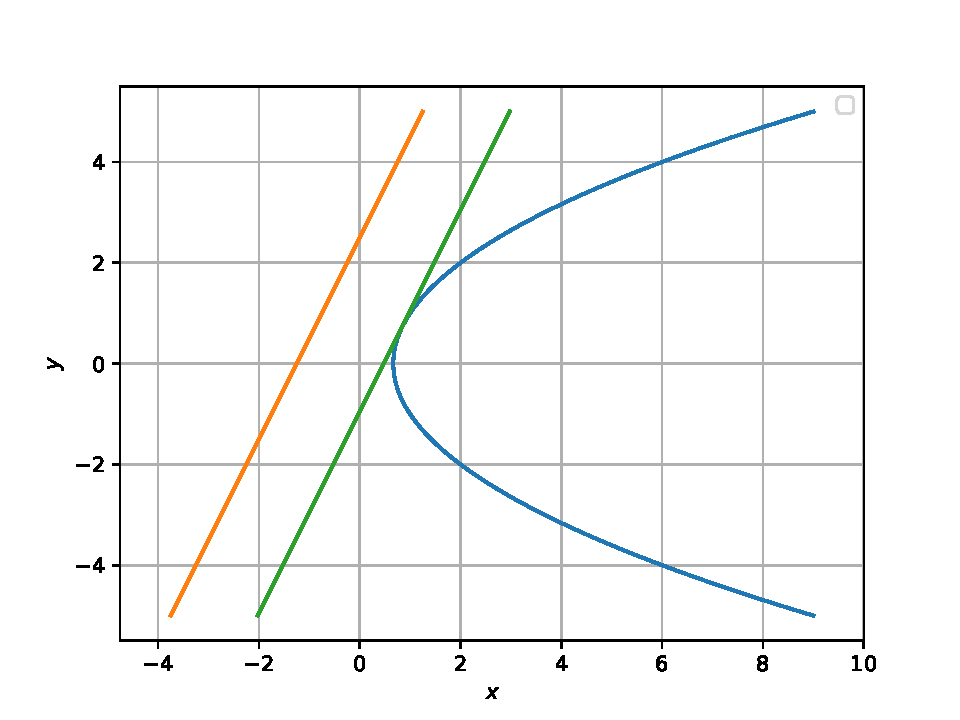
\includegraphics[scale=0.6]{../../../python/figs/conic.pdf} 
 \end{center}\vspace{1mm}
 
 \vspace{2mm} \textbf{Construction}
\begin{center}
\setlength{\arrayrulewidth}{0.5mm}
\setlength{\tabcolsep}{6pt}
\renewcommand{\arraystretch}{1.5}
    \begin{tabular}{|l|c|}
    \hline 
    \textbf{vertex} & \textbf{coordinates} \\ \hline
  $\vec{q}$ & $\myvec{
   at^2\\
   2at
   } $\\\hline
      \end{tabular}
  \end{center}
  
\raggedright  Download the code \\
Github link: \href{https://github.com/KrishnaYadati/Assignments/blob/main/Matrix_conic_assignment/codes/conic.py}{Assignment-6}.
  \end{multicols}
\end{document}
\fi

\section{Examples}
\subsection{Loney}

%We provide alternative solutions to the examples in \cite[p.336-352]{loney_coord}
%using the framework developed in this paper.
\begin{example}[parabola]
	To show that 
	%\cite[p.336]{loney_coord}
	\begin{align}
		9x^2 - 24xy + 16y^2-18x-101y+19=0
    \label{ex:parab}
	\end{align}
	is the equation of a parabola with latus rectum of length 3, vertex 
	\begin{align}
    \label{ex:parab-vertex}
		\frac{1}{25}\myvec{-29\\25}
	\end{align}
	and
	axis 
	\begin{align}
    \label{ex:parab-axis}
    3x-4y+7 = 0
	\end{align}
\end{example}
\solution 
	Comparing 
    \eqref{ex:parab}
with 
    \eqref{eq:conic_quad_form}, 
\begin{align}
    \label{ex:parab-V}
	\vec{V} &=\myvec{9 & -12 \\ -12 & 16}
\\
    \label{ex:parab-u}
	\vec{u} &= -\frac{1}{2}\myvec{18 \\ 101}
\\
    \label{ex:parab-f}
f &= 19
    \end{align}
    The eigenvalues of $\vec{V}$ are obtained as 
   % the solutions of 
\begin{align}
	\mydet{\lambda\vec{I}-\vec{V}} &=0
%	\mydet{\lambda-9 & 12 \\ 12 & \lambda-16} = 0
%	\\
	\\
	\implies 	
	%\lambda\brak{\lambda-25} &= 0 
	 \lambda_1 = 0, \lambda_2 = 25
	 \label{ex:parab-lam}
    \end{align}
    Since the $\vec{V}$ matrix has a 0 eigenvalue, 
    \eqref{ex:parab} is a parabola.
    The eigenvector corresponding to the 0 eigenalue is given by 
    \begin{align}
	    \myvec{9 & -12 \\ -12 & 16}\vec{p}_1 = \vec{0}
    \end{align}
    yielding
%    Row reducing the above matrix yields
    \begin{align}
%	     \xleftrightarrow[]{R_2 \leftarrow 3R_2 +4R_1 }
%			    \myvec{
%				    9 & -12
%			    \\
%			    0 & 0
%		    }
%		    \\
 \vec{p}_1 = \frac{1}{5}\myvec{4 \\ 3} 
	    \label{eq:parab-evec}
    \end{align}
    Substituting from 
    \eqref{ex:parab-V},
    \eqref{ex:parab-u},
    \eqref{ex:parab-f},
	    \eqref{eq:parab-evec}
    and 
	 \eqref{ex:parab-lam}
 in \eqref{eq:f0},
      \eqref{eq:eta} and 
			\eqref{eq:latus-ellipse}
			the latus rectum is obtained as
    \begin{align}
	    \eta &=\frac{\abs{2\vec{u}^{\top}\vec{p}_1}}{\lambda_2}
	   % \frac{\myvec{18 & 101}\myvec{4 \\ 3}}{25\times 5} 
	    = 3
    \end{align}
    The vertex of the parabola is obtained from 
    \eqref{eq:conic_parab_c} as 
  \begin{align}
%	    \myvec{ -\frac{1}{2}\myvec{18 & 101}+\frac{3}{10}\myvec{4 & 3} \\ \myvec{9 & -12 \\ -12 & 16}
%}\vec{c} 
%	  &= 
%	  \myvec{-19 \\ \frac{3}{10}\myvec{4 \\ 3}+\frac{1}{2}\myvec{18 \\ 101}}  
%\\
%	  \implies 
	  \myvec{	  -39 & -73  \\9 & -12  \\-12 & 16 }\vec{c} &= 
	  \myvec{  -19\\-21\\28}
	  %\text{or, } \vec{c} = 
	  %\myvec{ - \frac{29}{25}\\ \frac{22}{25}}
	  \label{ex:parab-c}
    \end{align}	
    yielding
    \eqref{ex:parab-vertex}.
    The second eigenvector of $\vec{V}$ is orthogonal to $\vec{p}_1$ and obtained as 
    \begin{align}
 \vec{p}_2 = \frac{1}{5}\myvec{3 \\ -4} 
    \end{align}
    Substituting from 
    \eqref{ex:parab-vertex}
and
	  \eqref{ex:parab-c}
    in 
	  \eqref{eq:major-minor-axis-quad}, the equation of the axis of symmetry for the parabola can be expressed as 
%    \begin{align}	
%	    \vec{p}_2\brak{\vec{x}-\vec{c}} &= 0
%	    \\
%	    \implies 
%	   \myvec{3 & -4}  \brak{\vec{x}-
%		\frac{1}{25}\myvec{-29\\25}
%	    } &= 0
%    \end{align}	
%    yielding 
    \eqref{ex:parab-axis}.



\begin{example}[ellipse]
	To show that the equation 
	%\cite[p.340]{loney_coord}
	\begin{align}
\label{ex:ellipse}
		14x^2 - 4xy + 11y^2-44x-58y+71=0
	\end{align}
	represents an ellipse with  centre
	\begin{align}
	    \label{ex:ellipse-center}
		\vec{c} = \myvec{2 \\ 3}
	\end{align}
	and lengths of semi-axes
	\begin{align}
		\label{eq:ellipse-semi-axis}
		\sqrt{6} \text{ and } 2
	\end{align}
\end{example}
\solution   The parameters for
\eqref{ex:ellipse}, 
are 
\begin{align}
	    \label{ex:ellipse-V}
	\vec{V} &=\myvec{14 & -2 \\ -2 & 11}
\\
	    \label{ex:ellipse-u}
	\vec{u} &= \myvec{22 \\ 29}
\\
f &= 71
	    \label{ex:ellipse-f}
    \end{align}
    Since 
    \begin{align}
	    \mydet{\vec{V}} = 150 > 0,
    \end{align}
\eqref{ex:ellipse} is an ellipse.  
Substituting from 
	    \eqref{ex:ellipse-V}
	    and 
	    \eqref{ex:ellipse-u}
	    in
    \eqref{eq:conic_nonparab_c},
the center of the ellipse is obtained as 
%    \begin{align}
%	    \vec{c} =	    \frac{1}{150}\myvec{11 & 2 \\ 2& 14}  
%	    \myvec{22 \\ 29}
%    \end{align}
%    yielding 
	    \eqref{ex:ellipse-center}.
Also, the eigenvalues of 
$\vec{V}$
are 
\begin{align}
	\lambda_1 = 10, 	\lambda_2 = 15
	    \label{ex:ellipse-lam}
    \end{align}
%    with respective eigenvectors
%\begin{align}
%	\vec{p}_1 &= \frac{1}{\sqrt{5}}\myvec{ 1 \\ 2}
%	\\
%	\vec{p}_2 &= \frac{1}{\sqrt{5}}\myvec{ -2 \\ 1}
%    \end{align}
%From  
%		\eqref{eq:ellipse-semi-axis},
%the axes of the ellipse are given by 
%\begin{align}
%	\myvec{ 1 & 2} \brak{\vec{x} - \myvec{2\\3}} &=0
%	\\
%	\myvec{ 2 &  -1} \brak{\vec{x} - \myvec{2\\3}} &=0
%    \end{align}
%
    Substituting
from 
	    \eqref{ex:ellipse-V},
	    \eqref{ex:ellipse-u}
	    and
	    \eqref{ex:ellipse-f}
	    in
	  \eqref{eq:major-minor-axis-quad},
    \begin{align}
	    f_0 
%	    &= \myvec{22 & 29}
%	    \frac{1}{150}\myvec{11 & 2 \\ 2& 14}
%	    \myvec{22 \\ 29}
%	    \\
	    &= 60
	    \label{ex:ellipse-f0}
    \end{align}
    Substituting from 
	    \eqref{ex:ellipse-lam}
	    and 
	    \eqref{ex:ellipse-f0}
	    in 
\eqref{eq:chord-len-major}
and
\eqref{eq:chord-len-minor}, 
    the lengths of the semi-axes are obtained as 
		\eqref{eq:ellipse-semi-axis}.

\begin{example}[hyperbola]
To show that the equation 
	%\cite[p.341]{loney_coord}
	\begin{align}
\label{ex:hyper} 
		x^2 - 3xy + y^2+10x-10y+21=0
	\end{align}
\end{example}
%
represents a hyperbola with centre
	\begin{align}
		\vec{c} = \myvec{-2 \\ 2}
	\end{align}
	and length of semi-axes
	\begin{align}
		\label{eq:hyper-semi-axis}
		\sqrt{2} \text{ and } \sqrt{\frac{2}{5}}
	\end{align}
\solution   The conic parameters for
\eqref{ex:hyper}, 
are 
\begin{align}
	    \label{ex:hyper-V}
	\vec{V} &=\frac{1}{2}\myvec{2 & - {3}\\- {3} & 2}
\\
	    \label{ex:hyper-u}
	\vec{u} &= \myvec{5\\-5}
\\
f &= 21
	    \label{ex:hyper-f}
    \end{align}
    Since 
    \begin{align}
	    \mydet{\vec{V}}  =  - \frac{5}{4} < 0,
    \end{align}
\eqref{ex:hyper} is a hyperbola.  
Substituting from 
	    \eqref{ex:hyper-V}
	    and 
	    \eqref{ex:hyper-V}
	    in
    \eqref{eq:conic_nonparab_c},
the center of the hyperbola is obtained as 
%    \begin{align}
%	    \vec{c} =-\frac{2}{5}\myvec{ {2} &  {3}\\ {3} &  {2}}  \myvec{5\\-5}
%    \end{align}
%    yielding 
	    \eqref{ex:ellipse-center}.
Also, the eigenvalues of 
$\vec{V}$
are 
\begin{align}
	\lambda_1 = - \frac{1}{2}, 	\lambda_2 =
 \frac{5}{2}
	    \label{ex:hyper-lam}
    \end{align}
%    with respective eigenvectors
%\begin{align}
%	\vec{p}_1 &= 
%    \frac{1}{\sqrt{2}}\myvec{1 \\ 1}
%	\\
%	\vec{p}_2 &= 
%     \frac{1}{\sqrt{2}}\myvec{- 1\\ 1}
%    \end{align}
%From  
%		\eqref{eq:hyper-semi-axis},
%the axes of the hyper are given by 
%\begin{align}
%	\myvec{ 1 & 2} \brak{\vec{x} - \myvec{2\\3}} &=0
%	\\
%	\myvec{ 2 &  -1} \brak{\vec{x} - \myvec{2\\3}} &=0
%    \end{align}

From 
	  \eqref{eq:major-minor-axis-quad},
    \begin{align}
	    f_0 
%	    \myvec{22 & 29}
%	    \frac{1}{150}\myvec{11 & 2 \\ 2& 14}
%	    \myvec{22 \\ 29}
%	    \\
	    &= -1
	    \label{ex:hyper-f0}
    \end{align}
    Substituting from 
	    \eqref{ex:hyper-lam}
	    and 
	    \eqref{ex:hyper-f0}
	    in 
\eqref{eq:chord-len-major}
and
\eqref{eq:chord-len-minor}, 
    the lengths of the semi-axes are then obtained as 
		\eqref{eq:hyper-semi-axis}.
\begin{example}[tangents]
To show that the tangents to the curve 
	%\cite[p.352]{loney_coord}
	\begin{align}
\label{ex:tangents} 
		x^2 + 4xy + 3y^2-5x-6y+3=0
	\end{align}
	parallel to the line 
	\begin{align}
\label{ex:tangents-line} 
x+4y+c = 0
	\end{align}
	are 
	\begin{align}
\label{ex:tangents-lines} 
		\begin{split}
		x+4y-5 &= 0
		\\
		x+4y-8 &= 0
		\end{split}
	\end{align}
\end{example}
\solution   The conic parameters for
\eqref{ex:tangents} 
are 
\begin{align}
	    \label{ex:tangents-V}
	\vec{V} &=\myvec{1 & 2\\2 & 3 }
\\
	    \label{ex:tangents-u}
	\vec{u} &= \myvec{- \frac{5}{2}\\-3}
\\
f &= 3
	    \label{ex:tangents-f}
    \end{align}
    Since 
    \begin{align}
	    \mydet{\vec{V}} = -1 < 0,
    \end{align}
\eqref{ex:tangents} is a hyperbola.  
    From 
\eqref{ex:tangents-line}, the normal vector to the tangent is 
    \begin{align}
	    \vec{n} = \myvec{1\\4} 
	    \label{ex:tangents-normal}
    \end{align}
    The equation of the tangent can be expressed as 
    \begin{align}
	    \vec{n}^{\top} \brak{  \vec{x}- \vec{q}_i }&= 0
    \end{align}
    where $\vec{q}_i$ are the points of contact.  Comparing the above with 
\eqref{ex:tangents-line},
    \begin{align}
	    c &= -\vec{n}^{\top} \vec{q}_i 
	    \label{ex:tangents-c}
    \end{align}
    which, upon substituting from 
\eqref{eq:conic_tangent_qk} can be expressed as 
    \begin{align}
	    c &= -\vec{n}^{\top} \cbrak{
		    \vec{V}^{-1}\brak{\kappa_i \vec{n}-\vec{u}}}
	    \\
	    &= -\vec{n}^{\top} \cbrak{
		    \vec{V}^{-1}\brak{
\pm \sqrt{
\frac{
f_0
}
{
\vec{n}^{\top}\vec{V}^{-1}\vec{n}
}
}\vec{n}-\vec{u}}}
\\
	    &=  
\pm \sqrt{
f_0
\vec{n}^{\top}\vec{V}^{-1}\vec{n}
}
+\vec{n}^{\top}\vec{V}^{-1}\vec{u}.
%\\
%	    &= - 
%		    \brak{
%\pm \sqrt{
%f_0
%\vec{n}^{\top}\vec{V}^{-1}\vec{n}
%}
%	    +\vec{n}^{\top}\vec{c}}
    \end{align}
%    upon substituting from 
%\eqref{eq:conic_tangent_qk}
%and 
%    \eqref{eq:conic_nonparab_c}
Substituting from 
	    \eqref{ex:tangents-V},
	    \eqref{ex:tangents-u}
	    and 
	    \eqref{ex:tangents-f}
	    in
      \eqref{eq:f0}, 
    \begin{align}
	    \vec{f}_0 % &=
	   % \myvec{ \frac{5}{2}\\3}
	   % \myvec{-3 & 2\\2 & -1}\myvec{ \frac{5}{2}\\3} - 3
	   % \\
	    &=- \frac{3}{4}
	    \label{ex:tangents-f0}
    \end{align}
    Substituing from 
	    \eqref{ex:tangents-V},
	    \eqref{ex:tangents-u},
	    \eqref{ex:tangents-normal}
	    and 
	    \eqref{ex:tangents-f0}
	    in 
	\eqref{eq:conic_normal_k}, 
    \begin{align}
	    c = -5 \text{ or  } c = -8 
	    \label{ex:tangents-ci}
    \end{align}
    yielding 
\eqref{ex:tangents-lines}.

\subsection{Miscellaneous}

\renewcommand{\theequation}{\theenumi}
%\begin{enumerate}[label=\arabic*.,ref=\theenumi]
\begin{enumerate}[label=\thesubsection.\arabic*.,ref=\thesubsection.\theenumi]
\numberwithin{equation}{enumi}
\item  Given unit basis vectors $\vec{a}, \vec{b}$, with angle	$\theta $ between them, the locus of the coordinates of a unit vector $\vec{c}$ in the space spanned by $\vec{a}, \vec{b}$  is given by 
		\begin{align}
\vec{x}^{\top}  \myvec{1 & \rho \\ \rho & 1}\vec{x} = 1
			\label{eq:misc-c-ellipse}
		\end{align}
			with $\rho = \cos \theta $.
\\
%		\begin{align}
%		\vec{V} = 	\myvec{1 & \cos \theta\\ \cos \theta & 1}, 
%			\label{eq:misc-locus}
%		\end{align}
		\solution Let 

		\begin{align}
			\vec{c}& =x_1\vec{a}+ x_2\vec{b} = \myvec{\vec{a} & \vec{b}}\vec{x}
		\end{align}
		Then, 
		\begin{align}
		\norm{\vec{c}}^2 &= \vec{x}^{\top}\myvec{\vec{a}^{\top} \\ \vec{b}^{\top}}\myvec{\vec{a} & \vec{b}}\vec{x}
\\
			&= \vec{x}^{\top}\myvec{1 & \vec{a}^{\top} \vec{b} \\ \vec{a}^{\top}\vec{b}& 1}\vec{x}
		\end{align}
			which can be expressed as 
			\eqref{eq:misc-c-ellipse}.
		\item Given the coordinates of $\vec{c}$, the angle $\theta$ between the  basis vectors 
			is given by
		\begin{align}
			\rho 
			= \frac{1 - \norm{\vec{x}}^2}{\vec{x}^{\top}\vec{R}\vec{x}}
			\label{eq:misc-c-ellipse-d-rho-final}
		\end{align}
		where 
		\begin{align}
			\vec{R}	&= \myvec{0 & 1 \\ 1 & 0}.
		\end{align}
%			by $\rho = \cos \theta$ in 
%			\eqref{eq:misc-c-ellipse-d-rho-final}.

		\solution Let 
		\begin{align}
			\vec{x} = \myvec{x_1 \\ x_2}
		\end{align}
For 
	  \begin{align}
		  \vec{V} = \myvec{1 & \rho \\ \rho & 1}, \vec{u} = 0, f = -1
	  \end{align}
	  in 
  \eqref{eq:conic_quad_form}, 
%		and 
		%\begin{align}
		%	\vec{x} = \myvec{x_1 \\ x_2}
		%\end{align}

		Since
		\begin{align}
			\mydet{\vec{V}} = 1-\rho^2, 
			0 < \mydet{\vec{V}} < 1,
		\end{align}
\eqref{eq:misc-c-ellipse}
		represents the equation of an ellipse.
		Using eigenvalue decomposition, 
		\begin{align}
			\vec{V} = \vec{P}^{\top}\vec{D}\vec{P}
		\end{align}
		where 
		\begin{align}
			\vec{P} = \frac{1}{\sqrt{2}}\myvec{1 & 1 \\ -1 & 1},
			\vec{D} = \myvec{1+\rho & 0 \\ 0 & 1-\rho}
		\end{align}
		Using the affine transformation, 
		\begin{align}
			\vec{x} = 
			\vec{P}\vec{y}
			\label{eq:misc-c-ellipse-affine}
		\end{align}
			\eqref{eq:misc-c-ellipse}
			can be expressed as 
		\begin{align}
			\vec{y}^{\top}\vec{D}\vec{y} &= 1
			\label{eq:misc-c-ellipse-d}
			\implies y_1^2\brak{1+\rho} + y_2^2\brak{1-\rho} &= 1
		\end{align}
		which can be simplified to obtain 
		\begin{align}
			\rho &= \frac{1 - y_1^2 -  y_2^2}{y_1^2 -  y_2^2}
			\\
			&= \frac{1 - \norm{\vec{y}}^2}{\vec{y}^{\top}\vec{Q}\vec{y}}
			\label{eq:misc-c-ellipse-d-rho}
		\end{align}
		where 
		\begin{align}
			\vec{Q}	&= \myvec{1 & 0 \\ 0 & -1}
		\end{align}
			From \eqref{eq:misc-c-ellipse-affine}, 
			\eqref{eq:misc-c-ellipse-d-rho} can be expressed as 
			\eqref{eq:misc-c-ellipse-d-rho-final}
			%\eqref{eq:misc-locus}.
		\begin{align}
\because \norm{\vec{a}} = \norm{\vec{b}} = 1.
		\end{align}

%		\begin{align}
%			\rho &= 			\cos \theta = \vec{a}^{\top} \vec{b} 
%\\
%			\implies \vec{x}^{\top}\vec{V}\vec{x} &= 1
%		\end{align}
%		where
%		\\
%			\label{eq:misc-c}
%			\\
%			&\brak
%		\end{align}
%		Letting  be the angle between $\vec{a}, \vec{b}$, 
%		\begin{align}
%			\rho &= 			\cos \theta = \vec{a}^{\top} \vec{b} 
%\\
%			\implies \vec{V} &= \myvec{1 & \rho \\ \rho & 1}, \abs{\rho} < 1
%		\end{align}
%		From 
%			\eqref{eq:misc-c}, since $\norm{\vec{c}} = 1$, 

%
%%\section*{Disclosure Statement}
%%The authors report there are no competing interests to declare.
%%
%%
%%
%%  
%%%All the results related to conics are summarized in 
%%%Table \ref{table:conics}.  
%%%\begin{table*}[!t]
%%%\centering
%%%\input{conics.tex}
%%%%\input{./figs/conics.tex}
%%%\caption{$\vec{x}^{\top}\vec{V}\vec{x}+2\vec{u}^{\top}\vec{x}+f = 0$  can be expressed in the above standard form for various conics. $\vec{c}$ represents the centre/vertex of the conic. $\vec{q}$ is/are the point(s) of contact for the tangent(s). }
%%%\label{table:conics}
%%%\end{table*}
%%%\begin{verbatim}
%%\bibliographystyle{tfs}
%%%\bibliography{interacttfssample}
%%\bibliography{school}
%%\end{verbatim}
%% included where the list of references is to appear, where \texttt{tfs.bst} is the name of the \textsc{Bib}\TeX\ bibliography style file for Taylor \& Francis' Reference Style S and \texttt{interacttfssample.bib} is the bibliographic database included with the \textsf{Interact}-TFS \LaTeX\ bundle (to be replaced with the name of your own .bib file). \LaTeX/\textsc{Bib}\TeX\ will extract from your .bib file only those references that are cited in your .tex file and list them in the References section.
%
%% Please include a copy of your .bib file and/or the final generated .bbl file among your source files if your .tex file does not contain a reference list in a \texttt{thebibliography} environment.
%

  % \section{Appendices}
  % \appendix
			\appendices
   \section{}

%\numberwithin{equation}{subsection}
\begin{definition}
	The {\em affine} transformation is given by 
    \begin{align}
	    \vec{x} &= \vec{P}\vec{y}+\vec{c} \quad \text{(Affine Transformation)}
\label{eq:conic_affine}
    \end{align}
	where $\vec{P}$ is invertible.
\end{definition}
\begin{definition}
	The eigenvalue decomposition of a symmetric matrix $\vec{V}$ is given by 
	%\cite{banchoff}
    \begin{align}
      \label{eq:conic_parmas_eig_def}
      \vec{P}^{\top}\vec{V}\vec{P} &= \vec{D}. \quad \text{(Eigenvalue Decomposition)}
      \\
      \vec{D} &= \myvec{\lambda_1 & 0\\ 0 & \lambda_2}, 
      \\
      \vec{P} &= \myvec{\vec{p}_1 & \vec{p}_2}, \quad \vec{P}^{\top}=\vec{P}^{-1},
      \label{eq:eigevecP}
    \end{align}
\end{definition}
\subsection{The Quadratic Form}
%\numberwithin{equation}{subsection}

\begin{definition}
  Let $\vec{q}$ be a point such that the ratio of its distance from a fixed point $\vec{F}$ and the distance ($d$) from a fixed line 
	\begin{align}
L: \vec{n}^{\top}\vec{x}=c 
	\end{align}
		is constant, given by 
\label{conics/30/def}
\begin{align}
\frac{\norm{\vec{q}-\vec{F}}}{d} = e    
\end{align}
The locus of $\vec{q}$ is known as a conic section. The line $L$ is known as the directrix and the point $\vec{F}$ is the focus. $e$ is defined to be 
the eccentricity of the conic.  
\begin{enumerate}
    \item For $e = 1$, the conic is a parabola
    \item For $e < 1$, the conic is an ellipse
    \item For $e > 1$, the conic is a hyperbola
\end{enumerate}
\end{definition}
\begin{theorem}
The equation of  a conic with directrix $\vec{n}^{\top}\vec{x} = c$, eccentricity $e$ and focus $\vec{F}$ is given by 
\begin{align}
    \label{eq:conic_quad_form}
    \vec{x}^{\top}\vec{V}\vec{x}+2\vec{u}^{\top}\vec{x}+f=0
    \end{align}
where     
\begin{align}
  \label{eq:conic_quad_form_v}
\vec{V} &=\norm{\vec{n}}^2\vec{I}-e^2\vec{n}\vec{n}^{\top}, 
\\
\label{eq:conic_quad_form_u}
\vec{u} &= ce^2\vec{n}-\norm{\vec{n}}^2\vec{F}, 
\\
\label{eq:conic_quad_form_f}
f &= \norm{\vec{n}}^2\norm{\vec{F}}^2-c^2e^2
%\\
    \end{align}
    
% \begin{align}
% \vec{x}^{\top}(t\vec{I}-\vec{n}\vec{n}^{\top})\vec{x}+2(c\vec{n}-t\vec{F})^{\top}\vec{x}+t\norm{\vec{F}}^2-c^2&=0
% \end{align}
%
%and 
% where 
% \begin{align}
%     %t=\frac{\norm{\vec{n}}^2}{e^2}
%     \norm{\vec{n}} = 1
% \end{align}
%\end{theorem}
\end{theorem}
\begin{proof}
  Using Definition \ref{conics/30/def} and Lemma \ref{conics/30/lemma},  for any point $\vec{x}$ on the conic,
\begin{align}
\norm{\vec{x}-\vec{F}}^2&=e^2 \frac{\brak{{\vec{n}^{\top}\vec{x} - c}}^2}{\norm{\vec{n}}^2}\label{conics/30/eq:1} \\
\implies \norm{\vec{n}}^2\brak{\vec{x}-\vec{F}}^{\top}\brak{\vec{x}-\vec{F}}&=e^2\brak{\vec{n}^{\top}\vec{x} - c}^2
\\
\implies \norm{\vec{n}}^2\brak{\vec{x}^{\top}\vec{x}-2\vec{F}^{\top}\vec{x}+\norm{\vec{F}}^2}&=e^2\brak{c^2+\brak{\vec{n}^{\top}\vec{x} }^2-2c\vec{n}^{\top}\vec{x}} \\
&=e^2\brak{c^2+\brak{\vec{x}^{\top}\vec{n}\vec{n}^{\top}\vec{x} }-2c\vec{n}^{\top}\vec{x}}
% t\vec{x}^{\top}\vec{x}-(\vec{n}^{\top}\vec{x} )^2-2t\vec{F}^{\top}\vec{x}+2c\vec{n}^{\top}\vec{x}=c^2-t\norm{\vec{F}}^2\\
% t\vec{x}^{\top}\vec{I}\vec{x}-\vec{n}^{\top}\vec{x} \vec{n}^{\top}\vec{x}+2(c\vec{n}-t\vec{F})^{\top}\vec{x}=c^2-t\norm{\vec{F}}^2\\
% \vec{x}^{\top}(t\vec{I}-\vec{n}\vec{n}^{\top})\vec{x}+2(c\vec{n}-t\vec{F})^{\top}\vec{x}+t\norm{\vec{F}}^2-c^2=0
\end{align}
%
which can be expressed as \eqref{eq:conic_quad_form} after simplification.

% See Appendix \ref{app:conicdef}
\end{proof}
\begin{theorem}
  The eccentricity, directrices and foci of \eqref{eq:conic_quad_form} are given by 
%  \eqref{eq:conic_quad_form_e} -
%  \eqref{eq:conic_quad_form_F} 
%  \begin{figure*}[!hb]
%	  \centering
%	  \hrule
\begin{align}
  \label{eq:conic_quad_form_e} 
  e&= \sqrt{1-\frac{\lambda_1}{\lambda_2}}
\\
\label{eq:conic_quad_form_nc} 
	\begin{split}
  \vec{n}&= \sqrt{\lambda_2}\vec{p}_1,  
  \\
	c &= 
  \begin{cases}
    \frac{e\vec{u}^{\top}\vec{n} \pm \sqrt{e^2\brak{\vec{u}^{\top}\vec{n}}^2-\lambda_2\brak{e^2-1}\brak{\norm{\vec{u}}^2 - \lambda_2 f}}}{\lambda_2e\brak{e^2-1}} & e \ne 1
    \\
    \frac{\norm{\vec{u}}^2 - \lambda_2 f   }{2\vec{u}^{\top}\vec{n}} & e = 1
  \end{cases}
	\end{split}
  \\
  \label{eq:conic_quad_form_F} 
  \vec{F}  &= \frac{ce^2\vec{n}-\vec{u}}{\lambda_2}
\end{align}  
%  \end{figure*}
\end{theorem}
\begin{proof}
	See Appendix \ref{app:conic-parameters}
\end{proof}

\begin{theorem}
\eqref{eq:conic_quad_form} represents 
	\begin{enumerate}
		\item a parabola for $\mydet{\vec{V}} = 0 $,
		\item ellipse for $\mydet{\vec{V}} > 0 $ and 
		\item hyperbola for $\mydet{\vec{V}} < 0 $.
	\end{enumerate}
%		\item a pair of straight lines if
%\begin{align}
%\mydet{
%\vec{V}&\vec{u}
%\\
%\vec{u}^{\top}&f
%}
%=  0, \quad \mydet{\vec{V}} < 0
%\label{eq:quad_forms_pair_det}
%\end{align}
%			else, it represents
\end{theorem}
\begin{proof}
  From \eqref{eq:conic_quad_form_e},
\begin{align}
  \frac{\lambda_1}{\lambda_2} = 1 - e^2
\end{align}
Also, 
\begin{align}
	\mydet{\vec{V}} =   \lambda_1\lambda_2 
\end{align}
	yielding Table \ref{table:det}
\begin{table}[!h]
\centering
%%%%%%%%%%%%%%%%%%%%%%%%%%%%%%%%%%%%%%%%%%%%%%%%%%%%%%%%%%%%%%%%%%%%%%
%%                                                                  %%
%%  This is the header of a LaTeX2e file exported from Gnumeric.    %%
%%                                                                  %%
%%  This file can be compiled as it stands or included in another   %%
%%  LaTeX document. The table is based on the longtable package so  %%
%%  the longtable options (headers, footers...) can be set in the   %%
%%  preamble section below (see PRAMBLE).                           %%
%%                                                                  %%
%%  To include the file in another, the following two lines must be %%
%%  in the including file:                                          %%
%%        \def\inputGnumericTable{}                                 %%
%%  at the beginning of the file and:                               %%
%%        \input{name-of-this-file.tex}                             %%
%%  where the table is to be placed. Note also that the including   %%
%%  file must use the following packages for the table to be        %%
%%  rendered correctly:                                             %%
%%    \usepackage[latin1]{inputenc}                                 %%
%%    \usepackage{color}                                            %%
%%    \usepackage{array}                                            %%
%%    \usepackage{longtable}                                        %%
%%    \usepackage{calc}                                             %%
%%    \usepackage{multirow}                                         %%
%%    \usepackage{hhline}                                           %%
%%    \usepackage{ifthen}                                           %%
%%  optionally (for landscape tables embedded in another document): %%
%%    \usepackage{lscape}                                           %%
%%                                                                  %%
%%%%%%%%%%%%%%%%%%%%%%%%%%%%%%%%%%%%%%%%%%%%%%%%%%%%%%%%%%%%%%%%%%%%%%



%%  This section checks if we are begin input into another file or  %%
%%  the file will be compiled alone. First use a macro taken from   %%
%%  the TeXbook ex 7.7 (suggestion of Han-Wen Nienhuys).            %%
\def\ifundefined#1{\expandafter\ifx\csname#1\endcsname\relax}


%%  Check for the \def token for inputed files. If it is not        %%
%%  defined, the file will be processed as a standalone and the     %%
%%  preamble will be used.                                          %%
\ifundefined{inputGnumericTable}

%%  We must be able to close or not the document at the end.        %%
	\def\gnumericTableEnd{\end{document}}


%%%%%%%%%%%%%%%%%%%%%%%%%%%%%%%%%%%%%%%%%%%%%%%%%%%%%%%%%%%%%%%%%%%%%%
%%                                                                  %%
%%  This is the PREAMBLE. Change these values to get the right      %%
%%  paper size and other niceties.                                  %%
%%                                                                  %%
%%%%%%%%%%%%%%%%%%%%%%%%%%%%%%%%%%%%%%%%%%%%%%%%%%%%%%%%%%%%%%%%%%%%%%

	\documentclass[12pt%
			  %,landscape%
                    ]{report}
       \usepackage[latin1]{inputenc}
       \usepackage{fullpage}
       \usepackage{color}
       \usepackage{array}
       \usepackage{longtable}
       \usepackage{calc}
       \usepackage{multirow}
       \usepackage{hhline}
       \usepackage{ifthen}

	\begin{document}


%%  End of the preamble for the standalone. The next section is for %%
%%  documents which are included into other LaTeX2e files.          %%
\else

%%  We are not a stand alone document. For a regular table, we will %%
%%  have no preamble and only define the closing to mean nothing.   %%
    \def\gnumericTableEnd{}

%%  If we want landscape mode in an embedded document, comment out  %%
%%  the line above and uncomment the two below. The table will      %%
%%  begin on a new page and run in landscape mode.                  %%
%       \def\gnumericTableEnd{\end{landscape}}
%       \begin{landscape}


%%  End of the else clause for this file being \input.              %%
\fi

%%%%%%%%%%%%%%%%%%%%%%%%%%%%%%%%%%%%%%%%%%%%%%%%%%%%%%%%%%%%%%%%%%%%%%
%%                                                                  %%
%%  The rest is the gnumeric table, except for the closing          %%
%%  statement. Changes below will alter the table's appearance.     %%
%%                                                                  %%
%%%%%%%%%%%%%%%%%%%%%%%%%%%%%%%%%%%%%%%%%%%%%%%%%%%%%%%%%%%%%%%%%%%%%%

\providecommand{\gnumericmathit}[1]{#1} 
%%  Uncomment the next line if you would like your numbers to be in %%
%%  italics if they are italizised in the gnumeric table.           %%
%\renewcommand{\gnumericmathit}[1]{\mathit{#1}}
\providecommand{\gnumericPB}[1]%
{\let\gnumericTemp=\\#1\let\\=\gnumericTemp\hspace{0pt}}
 \ifundefined{gnumericTableWidthDefined}
        \newlength{\gnumericTableWidth}
        \newlength{\gnumericTableWidthComplete}
        \newlength{\gnumericMultiRowLength}
        \global\def\gnumericTableWidthDefined{}
 \fi
%% The following setting protects this code from babel shorthands.  %%
 \ifthenelse{\isundefined{\languageshorthands}}{}{\languageshorthands{english}}
%%  The default table format retains the relative column widths of  %%
%%  gnumeric. They can easily be changed to c, r or l. In that case %%
%%  you may want to comment out the next line and uncomment the one %%
%%  thereafter                                                      %%
\providecommand\gnumbox{\makebox[0pt]}
%%\providecommand\gnumbox[1][]{\makebox}

%% to adjust positions in multirow situations                       %%
\setlength{\bigstrutjot}{\jot}
\setlength{\extrarowheight}{\doublerulesep}

%%  The \setlongtables command keeps column widths the same across  %%
%%  pages. Simply comment out next line for varying column widths.  %%
\setlongtables

\setlength\gnumericTableWidth{%
	80pt+%
	65pt+%
	70pt+%
	70pt+%
0pt}
\def\gumericNumCols{4}
\setlength\gnumericTableWidthComplete{\gnumericTableWidth+%
         \tabcolsep*\gumericNumCols*2+\arrayrulewidth*\gumericNumCols}
\ifthenelse{\lengthtest{\gnumericTableWidthComplete > \linewidth}}%
         {\def\gnumericScale{1*\ratio{\linewidth-%
                        \tabcolsep*\gumericNumCols*2-%
                        \arrayrulewidth*\gumericNumCols}%
{\gnumericTableWidth}}}%
{\def\gnumericScale{1}}

%%%%%%%%%%%%%%%%%%%%%%%%%%%%%%%%%%%%%%%%%%%%%%%%%%%%%%%%%%%%%%%%%%%%%%
%%                                                                  %%
%% The following are the widths of the various columns. We are      %%
%% defining them here because then they are easier to change.       %%
%% Depending on the cell formats we may use them more than once.    %%
%%                                                                  %%
%%%%%%%%%%%%%%%%%%%%%%%%%%%%%%%%%%%%%%%%%%%%%%%%%%%%%%%%%%%%%%%%%%%%%%

\ifthenelse{\isundefined{\gnumericColA}}{\newlength{\gnumericColA}}{}\settowidth{\gnumericColA}{\begin{tabular}{@{}p{90pt*\gnumericScale}@{}}x\end{tabular}}
\ifthenelse{\isundefined{\gnumericColB}}{\newlength{\gnumericColB}}{}\settowidth{\gnumericColB}{\begin{tabular}{@{}p{65pt*\gnumericScale}@{}}x\end{tabular}}
\ifthenelse{\isundefined{\gnumericColC}}{\newlength{\gnumericColC}}{}\settowidth{\gnumericColC}{\begin{tabular}{@{}p{70pt*\gnumericScale}@{}}x\end{tabular}}
\ifthenelse{\isundefined{\gnumericColD}}{\newlength{\gnumericColD}}{}\settowidth{\gnumericColD}{\begin{tabular}{@{}p{75pt*\gnumericScale}@{}}x\end{tabular}}

\begin{longtable}[c]{%
	b{\gnumericColA}%
	b{\gnumericColB}%
	b{\gnumericColC}%
	b{\gnumericColD}%
	}

%%%%%%%%%%%%%%%%%%%%%%%%%%%%%%%%%%%%%%%%%%%%%%%%%%%%%%%%%%%%%%%%%%%%%%
%%  The longtable options. (Caption, headers... see Goosens, p.124) %%
%	\caption{The Table Caption.}             \\	%
% \hline	% Across the top of the table.
%%  The rest of these options are table rows which are placed on    %%
%%  the first, last or every page. Use \multicolumn if you want.    %%

%%  Header for the first page.                                      %%
%	\multicolumn{4}{c}{The First Header} \\ \hline 
%	\multicolumn{1}{c}{colTag}	%Column 1
%	&\multicolumn{1}{c}{colTag}	%Column 2
%	&\multicolumn{1}{c}{colTag}	%Column 3
%	&\multicolumn{1}{c}{colTag}	\\ \hline %Last column
%	\endfirsthead

%%  The running header definition.                                  %%
%	\hline
%	\multicolumn{4}{l}{\ldots\small\slshape continued} \\ \hline
%	\multicolumn{1}{c}{colTag}	%Column 1
%	&\multicolumn{1}{c}{colTag}	%Column 2
%	&\multicolumn{1}{c}{colTag}	%Column 3
%	&\multicolumn{1}{c}{colTag}	\\ \hline %Last column
%	\endhead

%%  The running footer definition.                                  %%
%	\hline
%	\multicolumn{4}{r}{\small\slshape continued\ldots} \\
%	\endfoot

%%  The ending footer definition.                                   %%
%	\multicolumn{4}{c}{That's all folks} \\ \hline 
%	\endlastfoot
%%%%%%%%%%%%%%%%%%%%%%%%%%%%%%%%%%%%%%%%%%%%%%%%%%%%%%%%%%%%%%%%%%%%%%

\hhline{|-|-|-|-}
	 \multicolumn{1}{|p{\gnumericColA}|}%
	{\gnumericPB{\centering}\textbf{Eccentricity}}
	&\multicolumn{1}{p{\gnumericColB}|}%
	{\gnumericPB{\centering}\textbf{Conic}}
	&\multicolumn{1}{p{\gnumericColC}|}%
	{\gnumericPB{\centering}\textbf{Eigenvalue}}
	&\multicolumn{1}{p{\gnumericColD}|}%
	{\gnumericPB{\centering}\textbf{Determinant}}
\\
\hhline{|----|}
	 \multicolumn{1}{|p{\gnumericColA}|}%
	{\gnumericPB{\centering}$e = 1$}
	&\multicolumn{1}{p{\gnumericColB}|}%
	{\gnumericPB{\centering}Parabola}
	&\multicolumn{1}{p{\gnumericColC}|}%
	{\gnumericPB{\centering}$\lambda_1 =0$}
	&\multicolumn{1}{p{\gnumericColD}|}%
	{\gnumericPB{\centering}$\mydet{\vec{V}} = 0$}
\\
\hhline{|----|}
	 \multicolumn{1}{|p{\gnumericColA}|}%
	{\gnumericPB{\centering}$e < 1$}
	&\multicolumn{1}{p{\gnumericColB}|}%
	{\gnumericPB{\centering}Ellipse}
	&\multicolumn{1}{p{\gnumericColC}|}%
	{\gnumericPB{\centering}$\lambda_1 > 0, \lambda_2 > 0$}
	&\multicolumn{1}{p{\gnumericColD}|}%
	{\gnumericPB{\centering}$\mydet{\vec{V}} > 0$}
\\
\hhline{|----|}
	 \multicolumn{1}{|p{\gnumericColA}|}%
	{\gnumericPB{\centering}$e > 1$}
	&\multicolumn{1}{p{\gnumericColB}|}%
	{\gnumericPB{\centering}Hyperbola}
	&\multicolumn{1}{p{\gnumericColC}|}%
	{\gnumericPB{\centering}$ \lambda_1 < 0, \lambda_2 > 0$}
	&\multicolumn{1}{p{\gnumericColD}|}%
		{\gnumericPB{\centering}$\mydet{\vec{V}} < 0$}
\\
\hhline{|-|-|-|-|}
\end{longtable}

\ifthenelse{\isundefined{\languageshorthands}}{}{\languageshorthands{\languagename}}
\gnumericTableEnd

	\caption{}
\label{table:det}
\end{table}
\end{proof}


  \section{}

  \label{app:parab}
	Using 
\eqref{eq:conic_affine}
%such that 
\eqref{eq:conic_quad_form} can be expressed as

%\item  
%Substituting \eqref{eq:conic_affine} in \eqref{eq:conic_quad_form}
\begin{align}
\brak{\vec{P}\vec{y}+\vec{c}}^{\top}\vec{V}\brak{\vec{P}\vec{y}+\vec{c}}+2\vec{u}^{\top}\brak{\vec{P}\vec{y}+\vec{c}}+ f
	= 0, 
\end{align}
yielding 
\begin{align}
\vec{y}^{\top}\vec{P}^{\top}\vec{V}\vec{P}\vec{y}+2\brak{\vec{V}\vec{c}+\vec{u}}^{\top}\vec{P}\vec{y}
+  \vec{c}^{\top}\vec{V}\vec{c} + 2\vec{u}^{\top}\vec{c} + f= 0
\label{eq:conic_simp_one}
\end{align}
%
From \eqref{eq:conic_simp_one} and \eqref{eq:conic_parmas_eig_def},
\begin{align}
\vec{y}^{\top}\vec{D}\vec{y}+2\brak{\vec{V}\vec{c}+\vec{u}}^{\top}\vec{P}\vec{y}
+  \vec{c}^{\top}\brak{\vec{V}\vec{c} + \vec{u}}+ \vec{u}^{\top}\vec{c} + f= 0
\label{eq:conic_simp}
\end{align}
When $\vec{V}^{-1}$ exists, choosing
\begin{align}
%\begin{split}
\vec{V}\vec{c}+\vec{u} &= \vec{0}, \quad \text{or}, \vec{c} = -\vec{V}^{-1}\vec{u},
\label{eq:conic_parmas_c_def}
\end{align}
%
%%From \eqref{eq:conic_parmas_k_def} and 
%%
and substituting \eqref{eq:conic_parmas_c_def}
in \eqref{eq:conic_simp}
yields \eqref{eq:conic_simp_temp_nonparab}. 
	\subsection{}
%\item  
When $\abs{\vec{V}} = 0, \lambda_1 = 0$ and 
\begin{align}
\vec{V}\vec{p}_1 = 0, 
\vec{V}\vec{p}_2 = \lambda_2\vec{p}_2.
\label{eq:conic_parab_eig_prop} 
\end{align}
where $\vec{p}_1,\vec{p}_2$ are the eigenvectors of $\vec{V}$ such that  \eqref{eq:conic_parmas_eig_def}
%
\begin{align}
\vec{P} = \myvec{\vec{p}_1 & \vec{p}_2},
\label{eq:eig_matrix}
\end{align}
Substituting \eqref{eq:eig_matrix}
in \eqref{eq:conic_simp},
\begin{align}
	\vec{y}^{\top}\vec{D}\vec{y}+2\brak{\vec{c}^{\top}\vec{V}+\vec{u}^{\top}}\myvec{\vec{p}_1 & \vec{p}_2}\vec{y}
	+  \vec{c}^{\top}\brak{\vec{V}\vec{c} + \vec{u}}+ \vec{u}^{\top}\vec{c} + f&= 0
\\
\implies \vec{y}^{\top}\vec{D}\vec{y}
+2\myvec{\brak{\vec{c}^{\top}\vec{V}+\vec{u}^{\top}}\vec{p}_1  \brak{\vec{c}^{\top}\vec{V}+\vec{u}^{\top}}\vec{p}_2}\vec{y}
	+  \vec{c}^{\top}\brak{\vec{V}\vec{c} + \vec{u}}+ \vec{u}^{\top}\vec{c} + f&= 0
\\
\implies \vec{y}^{\top}\vec{D}\vec{y}
+2\myvec{\vec{u}^{\top}\vec{p}_1 & \brak{\lambda_2\vec{c}^{\top}+\vec{u}^{\top}}\vec{p}_2}\vec{y}
	+  \vec{c}^{\top}\brak{\vec{V}\vec{c} + \vec{u}}+ \vec{u}^{\top}\vec{c} + f&= 0
\end{align}
upon substituting from 
 \eqref{eq:conic_parab_eig_prop} yielding
\begin{align}
\lambda_2y_2^2+2\brak{\vec{u}^{\top}\vec{p}_1}y_1+  2y_2\brak{\lambda_2\vec{c}+\vec{u}}^{\top}\vec{p}_2
	+  \vec{c}^{\top}\brak{\vec{V}\vec{c} + \vec{u}}+ \vec{u}^{\top}\vec{c} + f= 0
\label{eq:conic_parab_foc_len_temp} 
\end{align}
%which is the equation of a parabola. 
Thus, \eqref{eq:conic_parab_foc_len_temp} 
can be expressed as \eqref{eq:conic_simp_temp_parab} by choosing
\begin{align}
%\label{eq:eta}
\eta = 2\vec{u}^{\top}\vec{p}_1
\end{align}
%Choosing 
%\begin{align}
%\vec{u} + \lambda_2\vec{c} = 0,
%\vec{c}^{\top}\brak{\vec{V}\vec{c} + \vec{u}}+ \vec{u}^{\top}\vec{c} + f = 0,
%\end{align}
% the above equation becomes
%\begin{align}
%y_2^2= -\frac{2\vec{u}^{\top}\vec{p}_1}{ \lambda_2} \brak{y_1
%+  \frac{\vec{u}^{\top}\vec{V}\vec{u} - 2\lambda_2\vec{u}^{\top}\vec{u} + f\lambda_2^2}{2\vec{u}^{\top}\vec{p}_1\lambda_2^2}}
%\\
%or \eta = 2\vec{u}^{\top}\vec{p}_1
%%\label{eq:conic_simp_parab_new}
%\end{align}
and $\vec{c}$ in \eqref{eq:conic_simp} such that
\begin{align}
\label{eq:conic_parab_one}
2\vec{P}^{\top}\brak{\vec{V}\vec{c}+\vec{u}} &= \eta\myvec{1\\0}
\\
\vec{c}^{\top}\brak{\vec{V}\vec{c} + \vec{u}}+ \vec{u}^{\top}\vec{c} + f&= 0
\label{eq:conic_parab_two}
\end{align}
%we obtain  \eqref{eq:conic_simp_temp_parab}.
$\because
\vec{P}^{\top}\vec{P} = \vec{I}$,
multiplying \eqref{eq:conic_parab_one} by $\vec{P}$ yields
\begin{align}
\label{eq:conic_parab_one_eig}
	\brak{\vec{V}\vec{c}+\vec{u}} &= \frac{\eta}{2}\vec{p}_1,
\end{align}
which, upon substituting in \eqref{eq:conic_parab_two}
results in 
\begin{align}
\frac{\eta}{2}\vec{c}^{\top}\vec{p}_1 + \vec{u}^{\top}\vec{c} + f&= 0
\label{eq:conic_parab_two_eig}
\end{align}
\eqref{eq:conic_parab_one_eig} and \eqref{eq:conic_parab_two_eig} can be clubbed together to obtain \eqref{eq:conic_parab_c}.

  \section{}

  \label{app:foc-dir}
%  \input{appendix.tex}
		\begin{enumerate}
			\item For the standard hyperbola/ellipse in \eqref{eq:conic_simp_temp_nonparab}, from 
					\eqref{eq:std-prm-P},
\eqref{eq:conic_quad_form_nc}
and 
					\eqref{eq:std-prm-u},
				\begin{align}
\label{eq:n-ell-hyp}
					\vec{n} &= \sqrt{\frac{\lambda_2}{f_0}} \vec{e}_1 
					\\
					c &= 
					%\pm \frac{\sqrt{-\lambda_2\brak{e^2-1}\brak{\lambda_2 f_0}}}{\lambda_2e\brak{e^2-1}}
					\pm \frac{\sqrt{-\frac{\lambda_2}{f_0}\brak{e^2-1}\brak{\frac{\lambda_2}{ f_0}}}}{\frac{\lambda_2}{f_0}e\brak{e^2-1}}
					\\
					&=\pm \frac{1}{e\sqrt{1-e^2}}
%					\\
%					&=\pm\sqrt{\abs{\frac{f_0}{\brak{1 - \frac{\lambda_1}{\lambda_2}}\frac{\lambda_1}{\lambda_2}}}}
\label{eq:c-ell-hyp}
				\end{align}
				yielding 
					\eqref{eq:dx-ell-hyp} upon substituting from 
\eqref{eq:conic_quad_form_e} and simplifying.
For the standard parabola in \eqref{eq:conic_simp_temp_parab},  from 
					\eqref{eq:std-prm-P},
\eqref{eq:conic_quad_form_nc}
and 
					\eqref{eq:std-prm-u}, noting that $f = 0$,

				\begin{align}
\label{eq:n-parab}
					\vec{n} &= \sqrt{\lambda_2} \vec{e}_1 
					\\
					c &=
	\frac{\norm{\frac{\eta}{2} \vec{e}_1}^2   }{2\vec{\brak{\frac{\eta}{2}} \brak{\vec{e}_1}^{\top}\vec{n}}} 
\\
					\\
					&= \frac{\eta}{4\sqrt{\lambda_2}}
\label{eq:c-parab}
				\end{align}
				yielding 
					\eqref{eq:dx-parab}.

				\item 	For the standard ellipse/hyperbola, substituting from
\eqref{eq:c-ell-hyp},
\eqref{eq:n-ell-hyp},
\eqref{eq:std-prm-u}
and \eqref{eq:conic_quad_form_e}
in \eqref{eq:conic_quad_form_F},
				\begin{align}
					\vec{F} &= \pm \frac{\brak{\frac{1}{e\sqrt{1-e^2}}}\brak{e^2}\sqrt{\frac{\lambda_2}{f_0}}\vec{e}_1}{\frac{\lambda_2}{f_0}}
					%\pm\sqrt{\abs{\frac{f_0}{\brak{1 - \frac{\lambda_1}{\lambda_2}}\frac{\lambda_1}{\lambda_2}}}}
					%\brak{1 - \frac{\lambda_1}{\lambda_2}}\frac{\sqrt{\lambda_2}}{\lambda_2}\vec{e}_1
 			\end{align}
			yielding
					\eqref{eq:F-ell-hyp-parab}
					after simplification.
					For the standard parabola, substituting from 
\eqref{eq:c-parab},
\eqref{eq:n-parab},
\eqref{eq:std-prm-u}
and \eqref{eq:conic_quad_form_e}
in \eqref{eq:conic_quad_form_F},			
				\begin{align}
	\vec{F}  &= \frac{\brak{\frac{\eta}{4\sqrt{\lambda_2}}}\sqrt{\lambda_2}\vec{e}_1-\vec{\frac{\eta}{2} \vec{e}_1}}{\lambda_2}
\\
				\end{align}
				yielding 
					\eqref{eq:F-ell-hyp-parab} after simplification.

		\end{enumerate}

		\section{}

		\label{app:major}
		Since the major axis passes through the origin, 
  \begin{align}
	  \vec{q} =			\vec{0} 
\end{align}  
Further, from Corollary  
		\eqref{corr:axis},
  \begin{align}
  \vec{m}&= \vec{e}_2,  
\end{align} and
from 
    \eqref{eq:conic_simp_temp_nonparab},
  \begin{align}
	  \vec{V} =     \frac{\vec{D} }{f_0}, 
	   \vec{u} = 0, 
	   f = -1
	    \label{eq:latus_rectum_ellipse_param}
\end{align}  
Substituting the above in
\eqref{eq:chord-len}, 
\begin{align}
 \frac{2\sqrt{
\vec{e}_1^{\top}\frac{\vec{D}}{f_0}\vec{e}_1
}
}
{
\vec{e}_1^{\top}\frac{\vec{D}}{f_0}\vec{e}_1
}\norm{\vec{e}_1}
  \end{align}
  yielding 
\eqref{eq:chord-len-major}.
Similarly, for the minor axis, the only different parameter is 
  \begin{align}
  \vec{m}&= \vec{e}_2,  
\end{align} 
Substituting the above in
\eqref{eq:chord-len}, 
\begin{align}
 \frac{2\sqrt{
\vec{e}_2^{\top}\frac{\vec{D}}{f_0}\vec{e}_2
}
}
{
\vec{e}_2^{\top}\frac{\vec{D}}{f_0}\vec{e}_2
}\norm{\vec{e}_2}
  \end{align}
  yielding 
\eqref{eq:chord-len-minor}.
		\section{}
		\label{app:latus}
			The latus rectum is perpendicular to the major axis for the standard conic.  Hence, from Corollary  
		\eqref{corr:axis},
  \begin{align}
  \vec{m}&= \vec{e}_2,  
\end{align}  
Since it passes through the focus, from 
					\eqref{eq:F-ell-hyp-parab}
  \begin{align}
	  \vec{q} =			\vec{F} 
=
					 \pm e\sqrt{\frac{f_0}{\lambda_2\brak{1-e^2}}} \vec{e }_1
%					 \frac{e}{\sqrt{f_0\lambda_2\brak{1-e^2}}}\vec{e }_1
\end{align}  
for the standard hyperbola/ellipse.  Also, 
from 
    \eqref{eq:conic_simp_temp_nonparab},
  \begin{align}
	  \vec{V} =     \frac{\vec{D} }{f_0}, 
	   \vec{u} = 0, 
	   f = -1
	    \label{eq:latus_rectum_ellipse_param-new}
\end{align}  
Substituting the above in
\eqref{eq:chord-len}, 
\begin{align}
 \frac{2\sqrt{
\sbrak{
\vec{e}_2^{\top}\brak{\frac{\vec{D}}{f_0} e\sqrt{\frac{f_0}{\lambda_2\brak{1-e^2}}} \vec{e }_1}
}^2
-
\brak
{
 e\sqrt{\frac{f_0}{\lambda_2\brak{1-e^2}}} \vec{e }_1^{\top}\frac{\vec{D}}{f_0} e\sqrt{\frac{f_0}{\lambda_2\brak{1-e^2}}} \vec{e }_1 -1 
}
\brak{\vec{e}_2^{\top}\frac{\vec{D}}{f_0}\vec{e}_2}
}
}
{
\vec{e}_2^{\top}\frac{\vec{D}}{f_0}\vec{e}_2
}\norm{\vec{e}_2}
\label{eq:chord-len-sub-ell}
  \end{align}
  Since 
  \begin{align}
\vec{e}_2^{\top}\vec{D}\vec{e}_1 = 0, 
%\vec{e}_2^{\top}\vec{e}_2 = 0,
\vec{e}_1^{\top}\vec{D}\vec{e}_1 = \lambda_1,
\vec{e}_1^{\top}\vec{e}_1 = 1,
	  \norm{\vec{e}_2} = 1,
\vec{e}_2^{\top}\vec{D}\vec{e}_2 = \lambda_2,
  \end{align}
\eqref{eq:chord-len-sub-ell} can be expressed as 
  \begin{align}
	&		\frac{2\sqrt{\brak{1-\frac{\lambda_1e^2}{{\lambda_2\brak{1-e^2}}}}\brak{\frac{\lambda_2}{f_0}}}}
{
	\frac{\lambda_2}{f_0}
	} 	
	\\
	&=		2\frac{\sqrt{
		f_0\lambda_1}}{\lambda_2}
 & \brak{ \because e^2 = 1-\frac{\lambda_1}{\lambda_2}}
		   \end{align}
For the standard parabola, the parameters in 
\eqref{eq:chord-len} are
\begin{align}  
	\vec{q} =\vec{F} =  -\frac{\eta}{4\lambda_2}\vec{e}_1, \vec{m} = \vec{e}_1, \vec{V} = \vec{D},
	\vec{u} = \frac{\eta}{2}\vec{e}_1^{\top}, f = 0
\end{align}  

Substituting the above in
\eqref{eq:chord-len}, 
%			from \eqref{eq:conic_simp_temp_nonparab},  
%					from \eqref{eq:F-ell-hyp-parab}
%and 						 \\
the length of the latus rectum  can be expressed as
{\footnotesize
\begin{align}
 \frac{2\sqrt{
\sbrak{
\vec{e}_2^{\top}\brak{\vec{D}\brak{-\frac{\eta}{4\lambda_2}\vec{e}_1}+\frac{\eta}{2}\vec{e}_1}
}^2
-
\brak
{
\brak{-\frac{\eta}{4\lambda_2}\vec{e}_1}^{\top}\vec{D}\brak{-\frac{\eta}{4\lambda_2}\vec{e}_1} + 2\frac{\eta}{2}\vec{e}_1^{\top}\brak{-\frac{\eta}{4\lambda_2}\vec{e}_1} 
}
\brak{\vec{e}_2^{\top}\vec{D}\vec{e}_2}
}
}
{
\vec{e}_2^{\top}\vec{D}\vec{e}_2
}\norm{\vec{e}_2}
\label{eq:chord-len-sub}
  \end{align}
  }
  Since 
  \begin{align}
\vec{e}_2^{\top}\vec{D}\vec{e}_1 = 0, 
\vec{e}_2^{\top}\vec{e}_2 = 0,
\vec{e}_1^{\top}\vec{D}\vec{e}_1 = 0,
\vec{e}_1^{\top}\vec{e}_1 = 1,
	  \norm{\vec{e}_1} = 1,
\vec{e}_2^{\top}\vec{D}\vec{e}_2 = \lambda_2,
  \end{align}
\eqref{eq:chord-len-sub} can be expressed as 
  \begin{align}
	  2 \frac{\sqrt{\frac{\eta^2}{4\lambda_2}\lambda_2}}{\lambda_2}
	  = \frac{\eta}{\lambda_2}
  \end{align}

%
\end{enumerate}

\end{document}
